\documentclass[letterpaper,11pt,openany]{book}

\usepackage{xmpincl}			% For including licensing XMP metadata
\usepackage{amsmath}			% AMS Math
%\usepackage{amssymb}			% AMS Symbol
\usepackage{fancyvrb}			% Fancy Verbatim
\usepackage{parskip}			% No indent, line skipping paragraph breaks. Comment for traditional breaks
\usepackage{float}				% For better control of figure placement and additional floats
\usepackage{subfig}				% For placing two images side by side in the same figure
\usepackage{caption}			% Caption controls for figures

\usepackage{fancyhdr}			% Fancy headers and footers. These will kick in the \mainmatter.
\pagestyle{empty}				% Empty for \frontmatter

\usepackage{graphicx}			% You know it, baby!
\graphicspath{{.}{content/images/}}

\usepackage{color}				% For link colors
\definecolor{linkcol}{rgb}{0,0,0.4} 
\definecolor{citecol}{rgb}{0.5,0,0}

\usepackage[bookmarksdepth=2,colorlinks=true,linkcolor=linkcol,citecolor=citecol,filecolor=magenta,urlcolor=linkcol,breaklinks=true]{hyperref}	% For all links within the document and URLs
\urlstyle{same}

\usepackage{minitoc}			% Mini table of contents for each chapter
\setcounter{minitocdepth}{2}

\usepackage[nottoc,notlof,notlot]{tocbibind}	% Fine tuning table of contents
\setcounter{tocdepth}{2}		% Number of levels shown in TOC
\setcounter{secnumdepth}{3}		% Levels of section numbering
\addtocontents{toc}{\protect\thispagestyle{empty}}		% Ensures no page
\addtocontents{lof}{\protect\thispagestyle{empty}}		% numbers on toc,
\addtocontents{lot}{\protect\thispagestyle{empty}}		% lof, or lot

%%%%%%%%%%%%%%%%%%%%%%%%%%%%%%%%% Definitions %%%%%%%%%%%%%%%%%%%%%%%%%%%%%%%%%
\hyphenation{me-di-um nano-par-ti-cles}

% Centered page environment for frontmatter. Credit to Matthieu Herrb (matthieu@laas.fr)
\newenvironment{vcenterpage}
{\newpage\vspace*{\fill}\thispagestyle{empty}\renewcommand{\headrulewidth}{0pt}}
{\vspace*{\fill}}

% Changes line spacing to be slightly easier to read
%\renewcommand{\baselinestretch}{1.05}

% Modifies book class defaults for better looking chapter pages with small caps titles
\makeatletter
\def\@makechapterhead#1{%
  \vspace*{1\p@}%
  {\parindent \z@ \raggedright \normalfont
    \ifnum \c@secnumdepth >\m@ne
      \if@mainmatter
        \LARGE\sc \@chapapp\space \thechapter
        \par\nobreak
        \vskip 10\p@
      \fi
    \fi
    \interlinepenalty\@M
    \Huge \sc #1\par\nobreak
    \vskip 25\p@
  }}
\def\@makeschapterhead#1{%
  \vspace*{1\p@}%
  {\parindent \z@ \raggedright
    \normalfont
    \interlinepenalty\@M
    \Huge \sc  #1\par\nobreak
    \vskip 30\p@
  }}
\makeatother
						% Packages and new defintions
\includexmp{base/CC_Attribution-NonCommercial-ShareAlike_2.5_Mexico}	% Licensing XMP metadata
\hypersetup{									% PDF display options
    pdftitle={Optical Nonlinear Spectroscopy of Gold and Silicon Nanoparticles},
    pdfauthor={Sean M. Anderson},
    pdfsubject={Nonlinear optical studies of gold and silicon nanoparticles using the XP2SHG/SFG technique.},
    pdfkeywords={nonlinear} {optics} {shg} {sfg} {nanoparticles} {spectroscopy} {surface} {techniques}}
    
%\usepackage{showkeys}							% Shows all \label values for quick troubleshooting

\usepackage[T1]{fontenc}						% T1 font encoding for special characters.
%\usepackage{lmodern}							% Better Latin Modern font.
\usepackage[bitstream-charter]{mathdesign}		% Charter BT fonts.

%\usepackage{draftwatermark}					% Add watermark to background
%\SetWatermarkText{DRAFT}
%\SetWatermarkScale{2}
%\SetWatermarkLightness{0.87}
%\SetWatermarkFontSize{2cm}

%\includeonly{}									% Select individual chapters for quicker drafts

\begin{document}
\dominitoc

\frontmatter
%\begin{titlepage}
\begin{center}
   {\href{http://www.cio.mx}{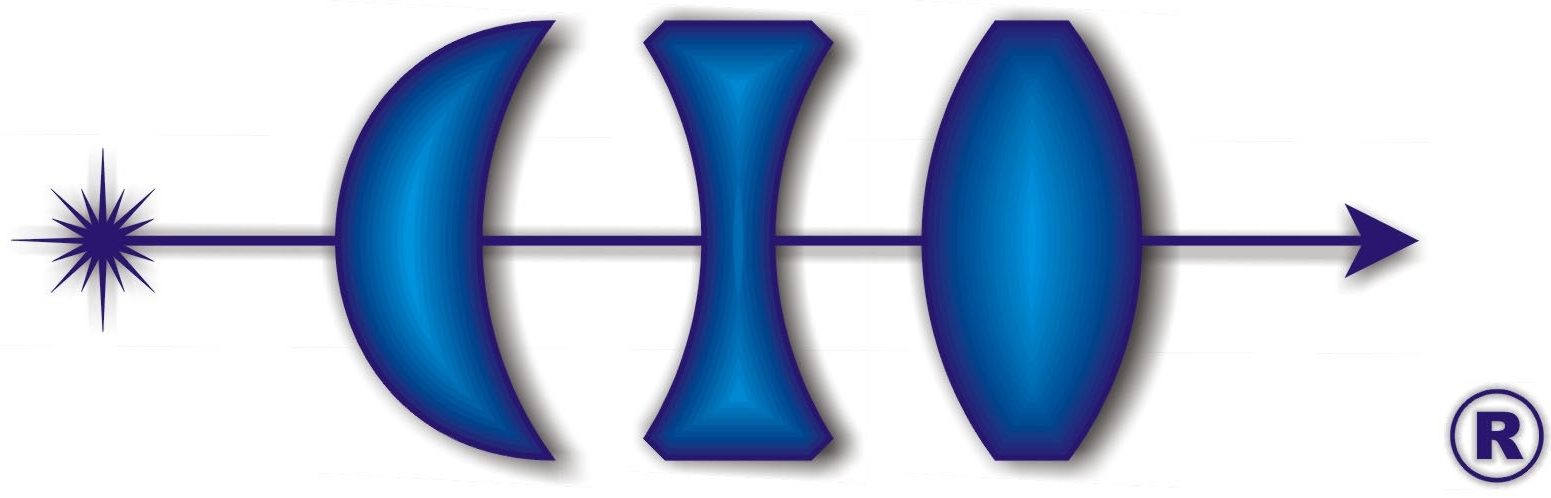
\includegraphics[scale=.7]{frontmatter/logo.png}}
   {\\
{{\href{http://www.cio.mx}{{{\Large Centro de Investigaciones en \'Optica}}, A.C.}}}\\   
    \vspace{.1cm}
 {\Large{Divisi\'on de Fot\'onica\\
\vspace{.1cm}
{{\small Loma del Bosque 115, Le\'on, Guanajuato, 37150, M\'exico}}
   }}}}
\vspace{2cm}

{\ttfamily
{\Huge{Optical Nonlinear Spectroscopy of Gold and Silicon Nanoparticles}}
\vspace{0.5cm}

{\large{by}}
\vspace{0.5cm}

{\LARGE{Sean M. Anderson}}
\vspace{0.5cm}
}

{\large A thesis submitted in partial fulfillment of the
                requirements \\for the degree of Master of Science (Optics).}

\vspace{2cm}

{\large\ttfamily{Advisor:\\ Dr.~Ram\'on Carriles Jaimes}}
\vfill
January 16, 2012
\end{center}
\end{titlepage}

			% Only for print version
\begin{titlepage}
\begin{center}
{\Huge Optical Nonlinear Spectroscopy of Gold and Silicon Nanoparticles}
\vspace{1.0cm}

{\large by}
\vspace{1.0cm}

{\LARGE Sean M. Anderson}
\vspace{3cm}

{\Large A thesis submitted in partial fulfillment of the requirements for the degree of Master of Science (Optics).}
\vspace{4cm}

{\large Advisor:\\
Dr.~Ram\'on Carriles Jaimes
\vspace*{1cm}

Divisi\'on de Fot\'onica\\
Centro de Investigaciones en \'Optica, A.C.\\
Loma del Bosque 115, Le\'on, Guanajuato, 37150, M\'exico}
\vfill
January 16, 2012
\end{center}
\end{titlepage}

\null
\vfill
\begin{flushleft}
The research presented in this thesis was carried out at the Centro de Investigaciones en \'Optica, A.C., Photonics Division, Loma del Bosque 115, Le\'on, Guanajuato, 37150, Mexico, and at the Femtosecond Spectroscopy Group, Department of Physics, University of Texas at Austin, 1 University Station, Austin, Texas, 78712, USA. Funding was provided by the CONACyT (Consejo Nacional de Ciencia y Tecnolog\'ia) in Mexico.

This thesis was made using only free and open source software (FOSS) with the exception of images not created by the author. It is typeset entirely using the \LaTeX{} Documentation System.
\vspace{1cm}

{\href{http://creativecommons.org/licenses/by-nc-sa/2.5/mx/}{
\includegraphics[scale=0.6]{frontmatter/by-nc-sa}}}

Copyright {\sffamily\copyright{}} 2012 by \href{http://www.roguephysicist.org}{Sean M. Anderson}.

This work is licensed under the Creative Commons Attribution-NonCommercial-ShareAlike 2.5 Mexico License. To view a copy of this license, visit \url{http://creativecommons.org/licenses/by-nc-sa/2.5/mx/} or send a letter to Creative Commons, 444 Castro Street, Suite 900, Mountain View, California, 94041, USA.
\end{flushleft}
\clearpage

\begin{center}
\vspace{2cm}
\noindent {\LARGE Optical Nonlinear Spectroscopy of Gold and Silicon Nanoparticles}\\
\vspace{0.7cm}
\noindent {\large by\\}
\vspace{0.7cm}
\noindent {\Large Sean M. Anderson}\\
\end{center}
\vfill
{\Large Approved:}
\begin{flushright}
\makebox[0.5\textwidth ]{\hrulefill}\\
\textbf{Dr. Ram\'on Carriles Jaimes}\\ Thesis Advisor
\vspace{1.25cm}

\makebox[0.5\textwidth ]{\hrulefill}\\
\textbf{Dr. Enrique Castro Camus}\\ Second Reader
\vspace{1.25cm}

\makebox[0.5\textwidth ]{\hrulefill}\\
\textbf{Dr. Bernardo Mendoza Santoyo}\\Third Reader
%\textbf{Dr. Norberte Arzate Plata}\\Third Reader
\vfill

\begin{center}
\large {Centro de Investigaciones en \'Optica, A.C.\\
January 16, 2012}
\end{center}
\end{flushright}

\vspace*{6cm}

%%%%%%%%%%
%{\huge Why must I treat the measuring device classically? What will happen to me if I don't?}

%\hfill {\large \emph{Eugene Paul Wigner}}

%%%%%%%%%%
{\LARGE One thing they don't tell you about doing experimental physics is that sometimes you must work under adverse conditions\ldots{} like a state of sheer terror.}

\hfill {\large \emph{W. K. Hartmann}}

%%%%%%%%%%
%{\huge Very strange people, physicists - in my experience the ones who aren't dead are in some way very ill.}

%\hfill {\large \emph{Douglas Adams}}

%%%%%%%%%%
%{\huge I refuse to answer that question on the grounds that I don't know the answer.}

%\hfill {\large \emph{Douglas Adams}}

%%%%%%%%%%
%{\huge If you wish to make an apple pie truly from scratch, you must first invent the universe.}

%\hfill {\large \emph{Carl Sagan}}

\begin{vcenterpage}
{\LARGE{\sc Abstract}}

\noindent\rule[2pt]{\textwidth}{0.5pt}
The primary focus of this thesis is the characterization of gold and silicon nanoparticles using second-order nonlinear optical spectroscopy. Nonlinear optical measurements are non-invasive and can provide information about surface and interface regions of materials. Nanoparticles have a very high surface to volume ratio, and second-order nonlinear optical phenomena are often produced from surface contributions, making them ideal methods for characterizing these nanostructures.

The two methods featured in this work are second harmonic generation (SHG) and sum frequency generation (SFG) with the two-beam, cross-polarized SHG/ SFG (XP2SHG/SFG) technique.

Optical characterization of nanoparticles and interfaces is currently a relevant topic in solid state and nano-scale physics. A non-destructive method for characterizing nano-materials is highly desirable and the XP2SHG/SFG technique is still relatively new for these types of materials.

\noindent\rule[2pt]{\textwidth}{0.5pt}
\end{vcenterpage}

\begin{vcenterpage}
{\LARGE{\sc Dedication}}

\noindent\rule[2pt]{\textwidth}{0.5pt}

I dedicate this thesis to my parents, Mike and Ana, and my love, Edith. Without them I would have never gotten this far.

\noindent\rule[2pt]{\textwidth}{0.5pt}
\end{vcenterpage}

\begin{vcenterpage}
{\LARGE{\sc Acknowledgements}}

\noindent\rule[2pt]{\textwidth}{0.5pt}

Big thanks go to my advisor Dr. Ram\'on Carriles for his exceptional patience and guidance throughout my extremely lethargic writing process. It is possible that his patience knows no bounds. His contribution to this work can be appreciated on every page.

I extend a huge acknowledgement to Dr. Mike Downer at UT Austin for allowing me to be a part of his research group for a month, and for the extra financial support he provided for me at no benefit to him. 

Very special thanks go to Junwei Wei, Ph.D. student at UT Austin for giving up his time helping me with the experimental part of my work. Without him none of this would have been possible. His skill and ability in the lab are amazing.

Dr. Bernardo Mendoza and Dr. Enrique Castro deserve great merit for accepting the torturous job of reviewing my work. I'd also like to thank Bernardo for accepting me into his Ph.D. group even after this!

My thanks go to Dr. Alejandro Reyes Esqueda of the UNAM for providing the samples used in this research.

I am very grateful towards the CONACyT for the financial support that allows a foreigner like me to study in an excellent institution like the CIO. I feel more at home in Mexico thanks to both institutions.

I would like to thank my close friends and blood brothers for all the good times had while I was arduously working on this thesis. Juan Jes\'us S\'anchez, Sergio Romero, Jos\'e Alberto Aguilar, and Marcelo Pereira kept me alert and ever vigilant -- whether in the office or at the \emph{Chemita}.

I also wish to thank my parents, Mike and Ana, for the considerable support they have given me throughout the years. They have always supported my endeavors in all possible ways.

Lastly, my most heartfelt gratitude goes towards my girlfriend Edith who motivated me to continue down this path in the first place. She has always given me the support and love needed to complete any goal I have set for myself, and I know that I can overcome any obstacle with her.

\noindent\rule[2pt]{\textwidth}{0.5pt}
\end{vcenterpage}


\tableofcontents
\listoffigures
%\listoftables

\mainmatter
% Fancy header style options for each page
\pagestyle{fancy}                       % Sets fancy header and footer
\fancyhead{}							% Resets headers
\fancyfoot{}							% and footers

\fancyhead[LE,RO]{\thepage}				% Page number left on even pages and right on odd pages
\fancyhead[RE]{\itshape\nouppercase{\leftmark}}		% Chapter right on even pages
\fancyhead[LO]{\itshape\nouppercase{\rightmark}}	% Section left on odd pages
\renewcommand{\headrulewidth}{0.5pt}

\fancypagestyle{plain}{
  \fancyhead{}
  \fancyfoot{}
  \renewcommand{\headrulewidth}{0pt}
}

% No headers on empty pages before new chapter
\makeatletter
\def\cleardoublepage{\clearpage\if@twoside \ifodd\c@page\else
    \hbox{}
    \thispagestyle{plain}
    \newpage
    \if@twocolumn\hbox{}\newpage\fi\fi\fi}
\makeatother \clearpage{\pagestyle{plain}\cleardoublepage}

\chapter[Introduction]{Introduction}\label{chap_intro}
\minitoc
\section{Motivation}
The principal motivation for this work is the analysis of different nanoparticles following two concepts:

\begin{description}
\item[First,] the use of second-order nonlinear optical effects that are very effective for surface analysis.
\item[Second,] the use of a special technique for optical spectroscopy -- the two beam, cross-polarized second harmonic/sum-frequency generation (XP2SHG/ SFG) technique. 
\end{description}

Metallic nanoparticles are currently a ``hot topic'' in the scientific world because the scope of their potential applications is very large, from biological applications \cite{baroli2007penetration}, imaging and detection \cite{lindfors2004detection, haick2007chemical, berciaud2006photothermal}, and more \cite{kamyshny2005ink, krenn1999squeezing}. Silicon nanoparticles, although more common, are not far behind -- their use in new solar cell technologies \cite{pillai2007surface} and biological markers \cite{li2004water} are also cutting edge research. 

None of the techniques described in this thesis are particularly new, but they have been used with great success in a variety of different materials. Although some literature exists on metallic nanoparticles characterized by these techniques, there is a relatively small amount of research on the subject. The optical methods included here are both non-destructive and potentially surface specific. Combining these with interesting nanostructures may prove to be a promising path for future developments in the nanosciences.

The focus of this thesis will be the study of second-order nonlinear effects in nanosystems. Nanoparticles have huge surface to volume ratios because they are so small; they contain few atoms and the bulk is tiny compared to the outside surface. The second-order nonlinearities, second harmonic generation (SHG) and sum-frequency generation (SFG), are both suitable for spectroscopic analysis of nanoparticles. These can be greatly enhanced using the two beam, cross-polarized SHG/SFG (XP2SHG/SFG) technique \cite{figliozzi2005single}. The purpose of this work is to study the properties of these nanostructures using the aforementioned methods.

\section{Nonlinear Optics in a Nutshell}\label{chap_intro_nonlin}
Linear optics has long dominated the study of light. Much like Newton's mechanics, it describes an incomplete picture of the interaction between light and the matter that forms our world. This is not to say the picture is incorrect; the interactions described work for our everyday situations. We call them ``linear'' because matter interacts in a directly proportional way with the electric field of the incoming light. The linear response of most materials is more appreciable than the other responses, making them difficult to observe -- we call these ``nonlinear effects.'' We will elaborate further on this point in chapter \ref{chap_theory}.

We can approximate most potentials within the atom using a harmonic oscillator model. These potentials represent the effect electrons feel when confined. They restrict the way electrons can move and determine many of the important material properties. These can tell us whether a material would make a good semiconductor for an optical device or for a computer microprocessor, or would make a very conductive metal, amongst many other things.

An example of a harmonic oscillator is a spring with a mass on one end. The other end is fixed and unmovable. If the mass is moved a little ways away from the equilibrium point and released, the mass will begin to oscillate for some time until it eventually stops once again at equilibrium (as it is dampened by gravity or friction). However, if you pull the spring too far it can deform from all the extra force. The spring follows a linear response according to the well established SHO equations when the displacement is small. Larger displacements are unaccounted for in this model -- now we are talking about \emph{nonlinear} behavior.

So the electrons behave in a similar manner if we model our electronic potentials as SHOs. This model works well for low intensities of incoming light, when the electron is displaced only a little from the ``bottom'' of the potential well. This provides the linear response between light and matter and is the reason why linear interactions dominate our everyday life. Although the light is very intense, the radiation that does reach us is spread out over half our world. Even when focused down to a very bright point it lacks the ability to deliver energy in an organized and efficient way. So our everyday light can only give electrons a little bit of energy and they move accordingly. Even the sun cannot provide the necessary conditions to allow electrons to move significantly from the bottom of a potential well.

We had the sun and different light bulbs, and used them often for experiments. I just explained why these sources can't help us past the linear regime. So people were stuck with this problem for a long time until a new light source, the LASER, was invented. LASER is an acronym for \emph{Light Amplification by Stimulated Emission of Radiation}. One of the main characteristics of a laser is that it emits an energetic, unidirectional, coherent beam of light that can be focused to a very small spot further concentrating the energy.

This discovery revolutionized optical science. The laser was precisely what was needed to produce high energy densities that could move the electrons away from the bottom of the potential well. Experimentalists starting shooting lasers into all kinds of materials -- and just like the spring and mass, the model stopped describing the experiment and all sorts of strange things started happening.

In this way we discovered nonlinear optics. These strange effects were difficult to explain at first. A new model had to be devised and tested against the experiments. Fortunately, it was not very long before one was created and found to work; not only did it explain everything observed until then, but it also predicted many things that had not yet been discovered \cite{boyd2003nonlinear, diels2006ultrashort, shen1984principles}. I will elaborate on the math of this new model in chapter \ref{chap_theory}.

SHG, a special case of SFG, was one of the first observed, and predominant optical nonlinearities that can appear from many substances. While all materials are technically nonlinear, the response of most are not appreciable for low intensities of incoming light, and are destroyed before we can see the effects. Some metals and semiconductors are excellent nonlinear materials, as are many different crystals. SHG is usually the first nonlinear effect to appear and can be the easiest to produce. As we will explain in section \ref{chap_theory_sum}, it is often attributed to surface emission which makes it an excellent tool for studying and characterizing surfaces and interfaces.

\section{Outline}
This thesis is divided into 5 chapters including this introduction. Chapter \ref{chap_theory} details the mathematics, formalism, and theory that make up our description of nonlinear optics. Chapter \ref{chap_setup} describes the materials to be characterized and the experimental setup used to study them. Chapter \ref{chap_results} consists of the experimental data and analysis, with comparisons to existing literature. Finally, chapter \ref{chap_conc} is dedicated to the final observations and remarks. The complete bibliography is located at the end of the document for easy reference.

\chapter{Nonlinear Optics and Nanoparticles}\label{chap_theory}
\minitoc
\section{A Review of Nonlinear Optics}
\subsection{Historical Overview}\label{chap_theory_hist}
The discovery of the optical maser by Townes \cite{PhysRev.112.1940} and the construction of the laser by Maiman in the late 1950s and early 1960s ushered a new age of optical discoveries. The ability to produce optical beams with these devices automatically lead to very highly focused energies distributed over very small areas. These concentrated energies allowed scientists to finally move into the optical nonlinear regime for many different materials.

The optical maser allowed for the first recorded observation of optical SHG by Franken et al. in 1961 \cite{PhysRevLett.7.118}. They produced a second beam of light at twice the frequency of the original by exciting a piece of crystalline quartz. This frequency doubling effect was dubbed SHG and was observed to be much less intense than the exciting beam.

There is a humorous anecdote about this experiment. Apparently, the editor of Physical Review Letters thought that the second harmonic dot on the photographic plate was a speck of dust, which he edited out. The image found in the article has an arrow pointing at the empty spot where it should be. However, this did not detract from the importance of the find.

Other developments followed promptly. In 1962, Bloembergen et al. \cite{PhysRev.127.1918, PhysRev.128.606} developed the mathematical framework to explain nonlinear optical phenomena. That same year, Terhune et al. \cite{PhysRevLett.8.404} observed SHG in calcite. These discoveries were amongst others \cite{lax1962nonlinear} that lead to further research into the geometrical dependence of nonlinear effects, and helped verify that the majority of the SHG signal produced in a centrosymmetric material comes from surface contribution, where inversion symmetry is broken.

In the late 1960s, Bloembergen \cite{PhysRev.174.813} and others \cite{PhysRev.178.1218} studied SHG in a variety of centrosymmetric materials and semiconductors. The advent of pulsed lasers during the 1970s \cite{nla.cat-vn2583352} allowed for even greater intensities to be obtained. Dye lasers came to prominence during these years, offering very large bandwidths and relatively short picosecond pulses. However, these lasers were very difficult to maintain and the dyes used were typically very toxic and presented serious health risks.

Interest began to form around using SHG to study surfaces and interfaces, since it had been proven \cite{PhysRevLett.46.145} to be exclusive to the surface area of a centrosymmetric material in the dipole approximation. Shen et al. published \cite{PhysRevB.38.7985} that there is also a quadrupole bulk contribution for this kind of material, and in 1989 \cite{shen89nature} published a review article summarizing most of the trends in surface spectroscopy using SHG. Theoretical work also played an important role in the 1990s, with new theoretical models by Sipe \cite{PhysRevB.53.10751} and others \cite{PhysRevB.53.4999, PhysRevB.60.14334, PhysRevB.55.2489, PhysRevB.57.2569}. Downer et al. \cite{downer2001optical} and L\"upke \cite{Lupke199975} both produced very thorough and referenced texts on SHG surface spectroscopy of semiconductors in the late 1990s and early 2000s. This period of time provided the foundations for surface optics today.

At around the same time, the first Ti:sapphire lasers were being produced and analyzed \cite{Moulton:86}. These early ultrafast lasers were capable of producing femtosecond pulses via mode-locked oscillators. Since the active medium is in solid state form, they present none of the risks of using dyes. These lasers were considerably more compact than dye lasers since they no longer needed external dye control systems. These lasers became commercial in the early 1990s.

Chirped pulse amplification (CPA) was invented in 1985 by Mourou and Strickland \cite{Strickland1985447}. This technique allowed Ti:sapphire lasers to achieve much higher peak energy without compromising the ultrashort pulse duration. During the 1990s, CPA became the prominent method for increasing energy output in Ti:sapphire lasers. At this point, Ti:sapphire lasers using the CPA technique were both compact, efficient, and cost effective. These factors would only improve over the following decade as the Ti:sapphire laser became the standard for high energy, ultrashort pulse applications.

\subsection{Defintion of Nonlinear Optics}
As explained briefly in section \ref{chap_intro_nonlin}, linear optics predominate in our everyday lives. The intensity of the light sources that surround us is typically not sufficient to modify the optical properties of a material. The discovery of the laser gave us access to higher intensity of polarized, directional, and coherent light. Beyond this, the ultrafast pulsed laser provides energy distributed into a much shorter time-frame which increases the peak irradiance delivered. These advances have greatly reduced the cost and effort needed to study nonlinear phenomena.

Light is nothing more than electromagnetic radiation, and is therefore composed of electromagnetic fields. This means that the study of how matter interacts with light is merely the study of how the light fields interact with the structure of matter. This can be readily appreciated for crystals and materials with very organized structures -- in fact, the best nonlinear materials are almost always crystalline in nature.

\subsubsection{Nonlinear Polarization and Susceptibility}
So what happens when very intense light coincides on a given material? Let us talk about the dipole moment per unit volume, or polarization $\mathbf{P}(t)$. This polarization describes the effect light has on a material and vice versa; it represents the optical response of a material.Taking Maxwell's equations with the usual considerations of zero charge density ($\rho=0$) and no free currents ($\mathbf{J}=0$), we have

\begin{align}
\nabla\cdot\mathbf{D} &= 0,\label{eq_max_1}\\
\nabla\cdot\mu_{0}\mathbf{H} &= 0,\\
\nabla\times\mathbf{E} &= -\mu_{0}\frac{\partial\mathbf{H}}{\partial t},\\
\nabla\times\mathbf{H} &= \frac{\partial\mathbf{D}}{\partial t}.
\end{align}

We take into account the nonlinearity of the material by relating the \textbf{D} and \textbf{E} fields with the total (linear and nonlinear) polarization \textbf{P},

\begin{equation}
\mathbf{D} = \epsilon_{0}\mathbf{E} + \mathbf{P}.
\end{equation}

Proceeding in the usual manner for deriving the wave equation, we obtain
\begin{equation}
\nabla\times\nabla\times\mathbf{E} + \frac{1}{c^{2}}\frac{\partial^{2}}{\partial t^{2}}\mathbf{E} = -\frac{1}{\epsilon_{0}c^{2}}\frac{\partial^{2}\mathbf{P}}{\partial t^{2}},
\end{equation}

which can be considerably simplified thanks to the identity
\begin{equation}
\nabla\times\nabla\times\mathbf{E} = \nabla\left(\nabla\cdot\mathbf{E}\right)-\nabla^{2}\mathbf{E}.
\end{equation}

The $\nabla\left(\nabla\cdot\mathbf{E}\right)$ term is usually negligible (for instance, if $\mathbf{E}$ is of the form of a transverse, infinite plane wave), so we can finally express the inhomogenous wave equation as
\begin{equation}
\nabla^{2}\mathbf{E} - \frac{1}{c^{2}}\frac{\partial^{2}}{\partial t^{2}}\mathbf{E} = \frac{1}{\epsilon_{0}c^{2}}\frac{\partial^{2}\mathbf{P}}{\partial t^{2}}.
\end{equation}

In this form, it is clear that the polarization acts as a source for this differential equation and we can recall our oscillator example from section \ref{chap_intro_nonlin}. The polarization can be expressed by a power series of the form
\begin{align}
{P}(t) &= \epsilon_{0}\left[\chi^{(1)}{E}(t) + \chi^{(2)}{E}^{2}(t) + \chi^{(3)}{E}^{3}(t) + \ldots\right]\label{eq_power}\\
			 &\equiv {P}^{(1)}(t) + {P}^{(2)}(t) + {P}^{(3)}(t) + \ldots,\label{eq_p_series}
\end{align}

where $\chi^{(n)}$ is the n\textsuperscript{th}-order susceptibility of the material. We can define the susceptibility as a constant of proportionallity that describes the degree of polarizability a material has in terms of the strength of an incoming optical electric field. The first term
\begin{equation}
P(t) = \epsilon_{0}\chi^{(1)}E(t),
\end{equation}

is the linear term that describes most everyday interactions between light and matter. When taking into account that the incoming fields are vectorial in nature, the linear susceptibility $\chi^{(1)}$ becomes a second-rank tensor. $\chi^{(2)}$, the second-order nonlinear optical susceptibility is a third-rank tensor \cite{boyd2003nonlinear}.

The nonlinear susceptibilities are very small in nature. If $\chi^{(1)}$ is unity, $\chi^{(2)}$ is on the order of $\approx 10^{-12}\,\text{m/V}$. This explains why such high intensity fields are needed to produce nonlinear interactions -- each term in equation \eqref{eq_power} depends on a higher power of the incoming field but has a much smaller value for the corresponding susceptibility.

A more general definition of the nonlinear polarization can be found when treating the input field as a superposition of plane waves. We assume that the electric field vector is of the form 
\begin{equation}
\mathbf{E}(\mathbf{r},t) = \sum_{n}\mathbf{E}_{n}(\mathbf{r},t),
\end{equation}

where
\begin{equation}
\mathbf{E}_{n}(\mathbf{r},t) = \mathbf{E}_{n}(\mathbf{r})e^{-i\omega_{n}t} + \text{c.c.}.
\end{equation}

If we look at the form of equation \eqref{eq_p_series}, we can express the nonlinear polarization in its full form as
\begin{equation}
\mathbf{P}(\mathbf{r},t) = \sum_{n}\mathbf{P}(\omega_{n})e^{-i\omega_{n}t}.
\end{equation}

Since we are only interested in second-order effects we can define the corresponding nonlinear polarization in terms of the second order susceptibility as
\begin{equation}
P_{i}(\omega_{n} + \omega_{m}) = \epsilon_{0}\sum_{jk}\sum_{(nm)}\chi^{(2)}_{ijk}(\omega_{n}+\omega_{m};\omega_{n},\omega_{m})E_{j}(\omega_{n})E_{k}(\omega_{m}),\label{eq_nonlin_p}
\end{equation}

where the indices $ijk$ refer to the Cartesian components of the fields, and $(nm)$ notes that $n$ and $m$ can be varied while the sum $\omega_{n} + \omega_{m}$ remains fixed.

We can study the generalized case when we have two incoming fields with frequencies $\omega_{1}$ and $\omega_{2}$. We can represent this in the following form
\begin{equation}
E(t) = E_{1}e^{-i\omega_{1}t} + E_{2}e^{-i\omega_{2}t} + \text{c.c.}\label{eq_sfg_form}
\end{equation}

Assuming the form of equation \eqref{eq_power}
\begin{equation}
P^{(2)} = \epsilon_{0}\chi^{(2)}E(t)^{2},
\end{equation}

and substituting expression \eqref{eq_sfg_form} we get
\begin{align}
P^{(2)}(t) &= \epsilon_{0}\chi^{(2)}\left[E^{2}_{1}e^{-i2\omega_{1}t} + E^{2}_{2}e^{-i2\omega_{2}t}\right.\nonumber\\
&+\left. 2E_{1}E_{2}e^{-i(\omega_{1}+\omega_{2})t} + 2E_{1}E^{\ast}_{2}e^{-i(\omega_{1}-\omega_{2})t} + \text{c.c.}\right]\nonumber\\
&+ 2\epsilon_{0}\chi^{(2)}\left[E_{1}E^{\ast}_{1} + E_{2}E^{\ast}_{2}\right].\label{eq_second_order}
\end{align}

We separate this expression into its components and the nonlinear effect that each represents in the following manner (abbreviations defined in table \ref{tab_janner}),
\begin{align}
P(2\omega_{1}) &= \epsilon_{0}\chi^{(2)}E^{2}_{1}e^{-i2\omega_{1}t} + \text{c.c.}\quad\text{(SHG)},\nonumber\\
P(2\omega_{2}) &= \epsilon_{0}\chi^{(2)}E^{2}_{2}e^{-i2\omega_{2}t} + \text{c.c.}\quad\text{(SHG)},\nonumber\\
P(\omega_{1}+\omega_{2}) &= 2\epsilon_{0}\chi^{(2)}E_{1}E_{2}e^{-i(\omega_{1}+\omega_{2})t} + \text{c.c.}\quad\text{(SFG)},\label{eq_list}\\
P(\omega_{1}-\omega_{2}) &= 2\epsilon_{0}\chi^{(2)}E_{1}E^{\ast}_{2}e^{-i(\omega_{1}-\omega_{2})t} + \text{c.c.}\quad\text{(DFG)},\nonumber\\
P(0) &= 2\epsilon_{0}\chi^{(2)}\left(E_{1}E^{\ast}_{1} + E_{2}E^{\ast}_{2}\right) + \text{c.c.}\quad\text{(OR)}.\nonumber
\end{align}

Janner \cite{janner1998exciton} has a wonderfully formatted table in her dissertation that summarizes the first few optical processes, which I reproduce here as follows.
\begin{table}[H]
\centering
\scalebox{0.9}{
\begin{tabular}{| c c c | p{6.5cm} | c |}
\hline
\multicolumn{3}{|c|}{$\quad\,\,\chi^{(n)}(-\omega;\omega_{1},\ldots,\omega_{n})$}	& Process & Order \\ \hline
$-\omega$ &;										& $\omega$				& Linear absorption / emission and refractive index									& 1 \\ \hline
$0$ & ; 											& $\omega,-\omega$		& Optical rectification (OR)															& 2 \\ \hline
$-\omega$ & ; & $0,\omega$													& Pockels effect																	& 2 \\ \hline
$-2\omega$ & ; & $\omega,\omega$											& Second-harmonic generation (SHG)													& 2 \\ \hline
$-(\omega_{1}+\omega_{2})$ & ; & $\omega_{1},\omega_{2}$					& Sum-frequency generation (SFG)													& 2 \\ \hline
$-(\omega_{1}-\omega_{2})$ & ; & $\omega_{1},\omega_{2}$					& Difference-frequency generation (DFG) / Parametric amplifcation and oscillation	& 2 \\ \hline
$-\omega$ & ; & $0,0,\omega$												& d.c. Kerr effect																	& 3 \\ \hline
$-2\omega$ & ; & $0,\omega,\omega$											& Electric Field induced SHG (EFISH)												& 3 \\ \hline
$-3\omega$ & ; & $\omega,\omega,\omega$										& Third-harmonic generation (THG)													& 3 \\ \hline
$-\omega$ & ; & $\omega,-\omega,\omega$										& Degenerate four-wave mixing (DFWM)												& 3 \\ \hline
$-\omega$ & ; & $-\omega_{2},\omega_{2},\omega_{1}$							& Two-photon absorption (TPA) / ionization / emission								& 3 \\ \hline
\end{tabular}}
\caption{Optical processes described by $\chi^{(n)}(-\omega;\omega_{1},\ldots,\omega_{n})$\label{tab_janner}}
\end{table}

From this point forward we will only be concerned with second-order effects.

\subsubsection{Symmetry Considerations for Centrosymmetric Materials}\label{chap_theory_sym}
As mentioned previously, $\chi^{(2)}$ is a third-rank tensor with 27 elements. The amount of non-zero elements varies with the symmetry properties of the medium. Knowing these properties can help us reduce the amount of unknown elements to calculate.

I will mention only one that proves to be of extreme importance for surface optics. A centrosymmetric material, or a material with an inversion center, is a material that for every point at coordinates $(x,y,z)$, there is an identical point located at $(-x,-y,-z)$. For instance, many crystals are centrosymmetric. If we assume that we are in the bulk of a centrosymmetric material, we can write the nonlinear polarization as
\begin{equation}
{P}(t) = \epsilon_{0}\chi^{(2)}{E}^{2}(t).\label{eq_regular}
\end{equation}

If the medium is centrosymmetric, a sign change must affect both the electric field and the polarization. So,
\begin{align}
-{P}(t) &= \epsilon_{0}\chi^{(2)}\left[-{E}(t)\right]^{2},\\
			  &= \epsilon_{0}\chi^{(2)}{E}^{2}(t).\label{eq_centro}
\end{align}

However, substituting \eqref{eq_centro} into \eqref{eq_regular} we get ${P}(t) = -{P}(t)$. We can finally deduce that
\begin{equation}
\chi^{(2)} = 0.
\end{equation}

Therefore, all second-order processes are forbidden in the bulk of centrosymmetric materials in the dipole approximation. We will talk about the other important approximation in section \ref{chap_theory_quad}. This property is broken at the surface since that region no longer presents an inversion center.  This very special property is what enables second-order nonlinearities to be so effective for surface and interface measurements. Likewise, any other mechanism that breaks the symmetry, such as an electric field or mechanical stress will also allow a second-order signal to be produced. See Bloembergen's \cite{bloembergen1999surface} excellent review about second-order effects for surface spectroscopy for further reading. 

\subsection{Bulk Quadrupolar and Other Contributions}\label{chap_theory_quad}
Everything that I have stated up to this point assumes what we call the \emph{dipole approximation} that arises from assuming that the polarization can take the form of a multipole expansion. The dipole approximation simply assumes that the dipolar contribution is significantly greater than all the others. This is not necessarily the case in many materials. In particular, we find that there can be a non-negligible electric quadrupole contribution from the bulk of centrosymmetric materials. Bloembergen et al. \cite{PhysRev.174.813} elaborate on this as early as the 1960s. This adds a severe complication to the use of second-order nonlinearities as surface probes since signal is actually produced from both surface and bulk. Sipe et al. \cite{sipe1987fundamental} go into some detail about this problem, stating that it is very difficult to separate the surface and bulk contributions as the various nonlinear coefficients cannot be measured separately. Guyot-Sionnest and Shen \cite{PhysRevB.38.7985} go one step further and state that the contributions are impossible to separate. They suggest that the best way to distinguish one from the other is by taking measurements before and after altering the surface and observing the overall changes to the produced signal. About a decade later, Shen et al. \cite{shen1999surface} state that bulk contributions not only come from the electric quadrupole, but also from the magnetic dipole, although the latter is typically much less intense than either of the former. They express the bulk polarization as a multipole series as follows,

\begin{equation}
\mathbf{P}^{B}(\omega) = \mathbf{P}_{D}(\omega) - \nabla\cdot\mathbf{Q}(\omega) - \left(\frac{c}{i\omega}\right)\nabla\times\mathbf{M}(\omega) + \ldots,
\end{equation}

where $\mathbf{P}_{D}(\omega)$ is the dipolar polarization, $\mathbf{Q}(\omega)$ is the electric quadrupole polarization, and $\mathbf{M}(\omega)$ is the magnetic dipole polarization. Indeed, if only the dipolar contribution is forbidden for centrosymmetric materials then there will be a contribution from the other two in addition to the dipolar contribution at the surface. The group does however go on to explain that there are a few experimental ways to help distinguish between surface and bulk contributions.

If $\mathbf{Q}(\omega)$ is assumed to take some form similar to

\begin{equation}
\mathbf{Q}(\omega) \approx \chi^{(2)}_{q}(\omega_{1} + \omega_{2})\mathbf{E}(\omega_{1})\nabla\mathbf{E}(\omega_{w}),
\end{equation}

then $\chi^{(2)}_{q}$ is a fourth-rank tensor with 81 independent elements. Clearly this adds some considerable complication to our problem and makes selecting the appropriate symmetry that much more important.

In summary, bulk electric quadrupole and magnetic dipole contributions to second-order surface effects may not be negligible and need to be taken into account. We will see later in sections \ref{chap_theory_nps} and \ref{chap_theory_xp2} that these considerations are important for studying nanoparticles when using the XP2SHG/SFG technique.

\subsection{SFG and SHG}\label{chap_theory_sum}
We call the third process in expression \eqref{eq_list} Sum-frequency generation (SFG). It is a second-order process that involves two photons, of frequencies $\omega_{1}$ and $\omega_{2}$ that combine to form one photon of frequency $\omega_{3} = \omega_{1} + \omega_{2}$. This is represented mathematically in the previous expression
\begin{equation}
P(\omega_{1}+\omega_{2}) = 2\epsilon_{0}\chi^{(2)}E_{1}E_{2}e^{-i(\omega_{1}+\omega_{2})t} + \text{c.c.},
\end{equation}

where the term is explicitly stated in the exponential. 

A special case of sum-frequency generation is when both incoming frequencies are the same, i.e. $\omega_{1} = \omega_{2}$. The resulting frequency is then exactly double that of the input frequency. 

As mentioned previously, second-order nonlinear processes are prohibited in the bulk of centrosymmetric materials (in the dipole approximation). Since it has a very strong surface contribution (where the inversion symmetry is broken), it can be used as a very precise diagnostic tool for surface and interface regions.

The use of these second-order nonlinearites for surface studies had gained momentum in the 1990s. McGilp wrote a review about using SHG and SFG as surface and interface probes in 1996 \cite{mcgilp1996review}. He adds experimental confirmation to his theories in 1999 \cite{mcgilp1999second} in an extremely thorough review about using SHG on the surface of almost any material you can think of. Aktsipetrov et al. \cite{aktsipetrov1997dc} followed a different approach by establishing what they call electric field induced second-harmonic generation, or EFISH. In this paper he elaborates how the sensitivity of SHG to surfaces can be enhanced by applying an electric field across the interface.

The theoretical side of things was further developed in a paper by Maytorena et al. \cite{PhysRevB.57.2569} discussing the formalities of SFG from surfaces by finding the exact expressions for the susceptibility based on modeling conductors and dielectrics. These models include fluid based, classical dynamics in addition to the wave equation treatment. A couple of interesting review papers by Downer et al. \cite{downer2001optical} and Scheidt et al. \cite{scheidt2004optical} exist, where they report results of SHG spectroscopies from a variety of different surfaces and interfaces including nanocrystals. These works are all predecessors for the later works we will discuss in section \ref{chap_theory_nps}.

\subsubsection{Phase-Matching}
What happens when the generated nonlinear wave propagates through a medium is that it becomes out of phase with the induced polarization after some distance. When this happens, the induced polarization will create new light out of phase with the light it created earlier and the two contributions will cancel out. This can be avoided if both frequencies of light (the fundamental and the produced second-order field) travel at the same phase velocity through the medium. Each wave with a different frequency will have a different wave-vector ($\mathbf{k}$) and wavenumber ($k$). Optimally, we would like a material such that

\begin{equation}
\Delta k = k_{1} + k_{2} - k_{3} = 0,\label{eq_phase}
\end{equation}

where $k_{1} = k_{2}$ for SHG. Equation \eqref{eq_phase} exemplifies a \emph{phase-matched} process. In practice, dispersion does not let this happen since the index of refraction of a material is almost never the same for different frequencies. There are certain materials that overcome this limitation (such as birefringent materials) that possess two indices of refraction.

Introducing equation \eqref{eq_phase} into the wave equation and solving, we can obtain the intensity profile \cite{boyd2003nonlinear} as

\begin{equation}
I(L) = \beta\,\vert P\vert^{2}\,L^{2}\text{sinc}^{2}\left(\frac{\Delta k L}{2}\right),
\end{equation}

where $L$ is the length of the material, $\Delta k$ is the phase mismatch, and $\beta$ are constants. The sinc function has a maximum at zero, so it is important to reduce the phase mismatch as much as possible. The inclusion of $L$ also indicates a relation to the material thickness. These considerations are important when selecting a nonlinear material such as a crystal -- most are sold in varying thicknesses that are optimized to work with certain frequencies.

In practice, phase-matching is usually improved through crystal orientation, selecting the right crystal thickness, and careful selection of the type of crystal being used.

\subsection{Optical Parametric Amplifiers}
We talked about how we can obtain different frequencies of light through wave mixing in section \ref{chap_theory_sum}. In practice however, it is considerably more difficult to implement a system in which we can easily create frequency addition or difference. It is no small task even with a fixed input wavelength. Most ultrafast lasers are tunable to some degree by adjusting internal components. We'll need something much more sophisticated if we want a variety of frequency choices.

An optical parametric amplifier (OPA) is a device that allows the user to obtain a wide bandwidth of wavelengths to work with, via the nonlinear processes of difference frequency generation (DFG) and optical parametric generation (OPG). Additionally, many commercial OPAs allow the user to tune the output by means of a motorized, computer-controlled interface. Some OPAs work on the basis of sum and difference frequency generation, using crystals to add and subtract the different frequencies in order to obtain the desired one.

OPG is a by-product of DFG. DFG occurs when a high frequency ($\omega_{1}$) photon is absorbed by an atom that jumps to a virtual level after being excited. It then decays producing two photons of lower frequency ($\omega_{2}$ and $\omega_{3}$). The creation of the $\omega_{2}$ photon is what we call OPG. If we instigate this process in the presence of an $\omega_{2}$ field, the same frequency ($\omega_{2}$) gets amplified at expense of the original $\omega_{1}$ photon. The $\omega_{3}$ frequency is called the idler and can be used in the same way as $\omega_{2}$ if desired. This effect is called optical parametric amplification. Therefore, we can create an OPA by creating a new frequency via OPG, and amplifying it using a crystal or other nonlinear media through optical parametric amplification. 

In practice most OPAs work like this: a high frequency, high power pump beam amplifies a lower frequency, lower power signal beam in a nonlinear crystal which is our desired $\omega_{2}$. This pump beam is usually the laser fundamental. This fixed pump beam transfers energy to produce the signal beam that is selectable via phase matching. This signal beam then feeds a second crystal to produce optical parametric amplification. We might be inclined to think that this is a form of stimulated emission similar to what happens in a laser (sans cavity). In stimulated emission, an electron drops from a higher level to a lower level due to the outside perturbing influence of an incident photon. It radiates with the exact same characteristics as the incoming field. OPA involves a transfer of energy from one photon to another (in our example, $\omega_{2}$ and $\omega_{1}$) to amplify $\omega_{2}$ while annihilating $\omega_{1}$.

\subsection{Noncollinear Optical Parametric Amplifiers}\label{chap_theory_nopa}
A noncollinear optical parametric amplifier (NOPA) replaces the $\omega_{2}$ signal with a white light super continuum. Tuning a NOPA is achieved by changing the angle between the seed and the pump beam, by changing the orientation of the crystal, or by using a delay stage to temporally overlap the fundamental with the desired frequency from the continuum.

In practice, the white light seed is typically generated from a sapphire window. The pump is normally the frequency doubled fundamental at 400 nm \cite{huber2001noncollinear, PhysRevB.84.165316}. The NOPA has a larger bandwidth than a regular OPA, and the resulting pulsewidth is dependent only on the bandwidth of the seed and not on the pulsewidth of the laser. For this reason, the NOPA has improved stability and spatial qualities. The added flexibility of the NOPA allows for different geometries to be implemented \cite{bodnar2010dual}. Gale \cite{gale1995sub} and Wilhelm et al. \cite{wilhelm1997sub} wrote some of the earliest papers refering to this type of OPA. Lee \cite{leecascaded} explains some of the formalism behind the operation of a NOPA.

\section{Second-Order Nonlinear Response of Nanoparticles}\label{chap_theory_nps}
The theory up to this point explains how second-order nonlinearities interact with matter and how they have been used for studying planar surfaces. I mentioned in chapter \ref{chap_intro} how nanoparticles have very large surface to volume ratios. The study of nanosystems with conventional optics has further motivated scientists to begin using second-order nonlinear phenomena to obtain more information from their samples.

I will briefly review some of the current models for describing the optical response for nanoparticles. These models consist of parametrizing the nonlinear response and then calculating the second-order emissions from the idealized nanosystem.

Dadap et al. \cite{dadap1999second} developed some early work in 1999, and later expanded on that in 2004 \cite{dadap2004theory}. They modeled SHG for a centrosymmetric nanosphere and concluded that SHG is produced via nonlocal excitation of the electric dipole moment and local excitation of the electric quadrupole moment. In other words, the electric-dipole can have excitation from either the electric quadrupole or the magnetic dipole, in addition to excitation provided by the incoming field. These results where verified experimentally by Shan et al. \cite{shan2006experimental} in an article from 2006, by taking angle- and polarization-resolved measurements of dye-coated polystyrene spheres. Brudny et al. \cite{brudny2000second} created a similar model that focuses on analytical expressions for the dipolar and quadrupolar second-order susceptibilities for a small dielectric sphere, and the nonlinear response for a Si sphere above a substrate.    

A more relevant treatment was published by Moch\'an et al. for an array of nanoparticles \cite{mochán2003second} that builds on their previous article \cite{brudny2000second}. This approach assumes spherical nanoparticles and should work well with the samples described in this work (see figures \ref{fig_tem_si_np} and \ref{fig_tem_gold_np}). I'll briefly review the method as follows.

\subsection{Theoretical Model}\label{mochan}
Let us assume a nanosphere centered at the origin. It has a linear response characterized in the usual way by its dielectric function $\epsilon(\omega)$. We assume the applied field, $\mathbf{E}^{\text{ex}}(\mathbf{r})$ is inhomogeneous and varies on a much larger scale than R, the radius of the nanoparticle. The dipole moment $\mathbf{p}^{(2)}$ is in some way related to $\mathbf{E}^{\text{ex}}(0)$ and $\nabla\mathbf{E}^{\text{ex}}(0)$, and is nonlocal as dictated by the symmetry of the sphere. We can express this relation as
\begin{equation}
\mathbf{p}^{(2)} = \gamma^{\rho}\mathbf{E}^{\text{ex}}(0)\nabla\cdot\mathbf{E}^{\text{ex}}(0) + \gamma^{e}\mathbf{E}^{\text{ex}}(0)\cdot\nabla\mathbf{E}^{\text{ex}}(0) + \gamma^{m}\mathbf{E}^{\text{ex}}(0)\times\left[\nabla\times\mathbf{E}^{\text{ex}}(0)\right],
\end{equation}

where $\gamma^{\rho}$, $\gamma^{e}$, and $\gamma^{m}$ are nonlinear response parameters. It is clearly nonlocal as it contains the field derivative. Likewise, \cite{brudny2000second} shows that the quadrupole moment, $\mathbf{Q}^{(2)}$, should be local, and symmetric of the form
\begin{equation}
\mathbf{Q}^{(2)} = \gamma^{q}\left(\mathbf{E}^{\text{ex}}(0)\mathbf{E}^{\text{ex}}(0) - \frac{1}{3}[\mathbf{E}^{\text{ex}}(0)]^{2}\,\mathbf{1}\right),
\end{equation}

where $\gamma^{q}$ is the parametric response parameter. Note that it is local and does not depend on the field derivative. As there is no external charge inside the sphere, $\gamma^{\rho} = 0$. A lengthy derivation is necessary to obtain the remaining response parameters and I will not include it here. From those parameters we obtain the values of $\mathbf{p}^{(2)}$ and $\mathbf{Q}^{(2)}$, with
\begin{equation}
Q^{(2)} = \gamma^{q}\left[\mathbf{E}^{\text{ex}}(0)\right]^{2}.
\end{equation}

Substituting these into the expression for the macroscopic nonlinear polarization for the entire array of spheres
\begin{equation}
\mathbf{P}^{nl} = n_{s}\mathbf{p}^{(2)} - \frac{1}{6}\nabla\cdot n_{s}\mathbf{Q}^{(2)} - \frac{1}{6}\nabla n_{s}Q^{(2)},
\end{equation}

where $n_{s}$ is the nanocrystal volume density; we can then obtain
\begin{equation}
\mathbf{P}^{nl} = \Gamma\nabla E^{2} + \Delta^{\prime}\left(\mathbf{E}\cdot\nabla\mathbf{E}\right).
\end{equation}

The first term can be neglected because it is longitudinal and does not radiate. With $\Delta^{'}\equiv n_{s}\left(\gamma^{e} - \gamma^{m} - \gamma^{q}/6\right)$, we can finally write the expression for the polarization as
\begin{equation}
\mathbf{P}^{(2)} = \Delta^{\prime}\left(\mathbf{E}\cdot\nabla\mathbf{E}\right),\label{eq_mochan_p}
\end{equation}

where $\mathbf{E}$ represents the incoming laser field. The relevance of this expression will become apparent in section \ref{chap_theory_xp2}, when we discuss the XP2SHG/SFG technique.

\subsection{Other Works}
Two relatively recent articles have studied different nonlinear effects on a variety of nanoscale gold shapes (primarily split-ring resonators) \cite{klein2007experiments, feth2008second}. The group hypothesizes that the samples show improved SHG due to local and nonlocal fields; in this case, magnetic resonances.

Zeng et al. \cite{zeng2009classical} developed a model based on classical electrodynamics to predict SHG in metallic nanostructures. Solving Maxwell's equations yields an expression for the SHG signal intensity and is surprisingly close to experimental values. However, the derivation is considerably easier due to the approximations.

For further reading, Link and El-Sayed \cite{link2003optical} offer a very extensive review of many other optical properties of nanoparticles.

\subsection{Summary}
In this section we saw how the theory indicates that the second-order response of nanoparticles depends both on the strength of the incoming field, but also on its characteristics. We also introduced the dependence on $\left(\mathbf{E}\cdot\nabla\right)\mathbf{E}$ of the nonlinear second-order polarization. With this information in hand we can determine the best technique to optimize our nonlinear signal.

Formally, we learned that the second-order nonlinearities are produced in nanoparticles thanks to local interface electric dipole contributions, plus quadrupolar contributions from the interior of the nanoparticles.

\section{Theory for the XP2SHG/SFG Technique}\label{chap_theory_xp2}
In 2003, Cattaneo and Kauranen \cite{cattaneo2003determination} published about a promising new technique involving two beams coinciding on a thin film. They proposed that the use of the second beam reduces the number of nonlinear coefficients to be determined if the polarization of the two beams is properly described beforehand. The method was simple enough -- they expressed the parallel and perpendicular fields separately as a sum of expansion coefficients that are in themselves linear combinations of susceptibility components. Changing the polarization of the control and probe beam would determine different coefficients. Adding the linear optical properties of the film and modeling with Green's-function led to the desired $\chi^{(2)}$ coefficients.

Following in 2005, Figliozzi et al. \cite{figliozzi2005single} note the importance of the aforementioned $\left(\mathbf{E}\cdot\nabla\mathbf{E}\right)$ term and relate it to the enhanced quadrupolar contribution; they go on to experimentally verify that dependence. They also discover that the two beam arrangement greatly enhances the entire SHG signal, both from the microscopic contributions of the particles as well as the bulk quadrupolar contribution from the substrate. This brings up the issue of how to discriminate between the two contributions to the SHG signal, which they manage to do by contrasting the difference in signal at different polarizations between the particles and the unimplanted glass.

In 2009 Wang et al. with some of the same people from references \cite{klein2007experiments} and \cite{feth2008second} elaborate a study on a gold thin film using a two-beam configuration \cite{wang2009surface}. They follow a similar model to that described in \cite{figliozzi2005single}, but their goal is separating the surface and bulk components of the SH field. This is done by finding material parameters due to the magnetic dipole and electric quadrupole by varying the polarization of the incoming beams. They succeed in finding which components of $\chi^{(2)}$ belong to surface only, bulk only, or both.

A very recent and thorough article \cite{PhysRevB.84.165316} by Wei et al. presents experimental evidence that supports the use of two-beam SHG with nanoparticles. They go into detail about the linear characterization of the Si nanocrystals used, which includes photoluminescence spectra, spectroscopic ellipsometry, and Raman microspectroscopy. By moving the sample across the overlapping beam region (the Z-scan technique) they were able to effectively determine which signal was produced by nanoparticles and which by bulk contributions from the substrate. They conclude with a very complete characterization of the Si nanocrystals after comparing the obtained data with that of the other conventional spectroscopies. Coincidentally, the setup described in this article is the exact one used in the experimental portion of this work, and is detailed in chapter \ref{chap_setup}.

A 2008 article \cite{wirth2008second} by Wirth et al. provides excellent review of the exact technique used in this work. It is also noteworthy in that it is the first article to refer to this technique as XP2SHG. Following on the work that we discussed in section \ref{mochan}, they establish that the polarization of the samples can be separated into two expressions,

\begin{align}
\mathbf{P}^{(2)}_{nc} &\equiv n_{b}\left(\gamma^{e}-\gamma^{m}-\frac{\gamma^{q}}{6}\right)\left(\mathbf{E}\cdot\nabla\right)\mathbf{E},\label{eq_p_nc}\\
\mathbf{P}^{(2)}_{g} &\equiv \left(\delta-\beta- 2\gamma\right)\left(\mathbf{E}\cdot\nabla\right)\mathbf{E},
\end{align}

where equation \eqref{eq_p_nc} is identical to \eqref{eq_mochan_p}. The article confirms that the XP2SHG technique enhances both the nanocrystal and glass signals, and goes on to say that the detected SHG signal is a product of the interference of both. This would account for shape of the plotted data from the results of the Z-scan presented in \cite{wirth2008second}, in \cite{PhysRevB.84.165316}, and in chapter \ref{chap_results} of this thesis.

The fields can be described by the amplitudes of the SH field from the nanocrystals $\vert\Gamma_{nc}\vert$, the glass $\Gamma_{g}$, and the phase $\Phi$ between them such that

\begin{align}
\mathbf{P}^{(2)}_{nc} &\equiv \vert\Gamma_{nc}\vert e^{i\Phi}\left(\mathbf{E}\cdot\nabla\right)\mathbf{E},\\
\mathbf{P}^{(2)}_{g} &\equiv \Gamma_{g}\left(\mathbf{E}\cdot\nabla\right)\mathbf{E}.
\end{align}

Three independent Z-scan measurements are needed to enable isolation of the nanocrystal signal and obtain the three unknowns $\vert\Gamma_{nc}\vert, \Gamma_{g}$, and $\Phi$: a glass scan, a scan with the nanocrystals at the entrance position, and with the nanocrystals at the exit position. They establish an empirical model based on the wave equations for each measurement, thus determining the intensity profile expressions in terms of the unknowns. All that is left is running the scans and plugging in the data to determine them and fully isolate the different contributions.

Studies like those included in \cite{PhysRevB.84.165316} and \cite{wirth2008second} are precisely in line with the work presented in this thesis.

\subsection{Signal enhancement with XP2SHG/SFG}
It was confirmed \cite{figliozzi2005single, sun2005quadrupolar} by Sun and Figliozzi et al. that the dipolar SHG single beam count rate scales as

\begin{equation}
N_{SHG} \sim f_{\text{rep}}I^{2}A\tau = \frac{f_{\text{rep}}\mathcal{E}^{2}}{\tau A},
\end{equation}

where $A$ is the beam spot size ($A = \pi w^{2}_{0}$), $\tau$ is the pulse duration, $\mathcal{E}$ is the pulse energy, and $f_{\text{rep}}$ is the repetition rate of the pulses. In correlation with the $\left(\mathbf{E}\cdot\nabla\right)\mathbf{E}$ dependence, that same group determined that the derivative creates an additional term for a Gaussian beam. This term comes from the quadrupolar contribution and introduces an extra factor of $A$, such that

\begin{equation}
N_{SHG} \sim \frac{f_{\text{rep}}\mathcal{E}^{2}}{\tau A^{2}}.
\end{equation}

If we use two incoming plane wave fields, we obtain from \eqref{eq_p_nc} (ignoring constants)

\begin{equation}
\mathbf{P}^{(2)}_{nc} \approx \left[(\mathbf{E}_{1}\cdot\nabla)\mathbf{E}_{2} + (\mathbf{E}_{2}\cdot\nabla)\mathbf{E}_{1}\right]e^{i(\mathbf{k}_{1} + \mathbf{k}_{2})\cdot\mathbf{r}}.
\end{equation}

We define the incoming fields as

\begin{equation}
\mathbf{E}_{i}(\mathbf{r}) = \hat{\epsilon}_{i}\mathcal{E}e^{i\mathbf{k}_{i}\cdot\mathbf{r}},
\end{equation}

where $\hat{\epsilon}_{i}$ is the polarization. For \emph{cross-polarized} beams, $\hat{\epsilon}_{1}\perp\hat{\epsilon}_{2}$; if $\hat{\epsilon}_{1} = \hat{y}$, then

\begin{equation}
\mathbf{P}^{(2)}_{nc} \approx \frac{1}{\lambda}\mathcal{E}_{1}\mathcal{E}_{2}\sin\alpha\hat{y},
\end{equation}

where $\frac{1}{\lambda} = k$. Now the signal intensity scales as 

\begin{equation}
N_{SHG} \sim \frac{f_{\text{rep}}\mathcal{E}_{1}\mathcal{E}_{2}\sin^{2}\alpha}{\lambda^{2}\tau A^{2}},
\end{equation}

where $\alpha$ is the angle between the beams. The $\frac{1}{\lambda}^{2}$ factor increases the intensity of the signal very significantly, while the $\sin^{2}\alpha$ term allows us to optimize the beam angle.

\subsection{Summary}
We used this section to discuss the fine points behind the XP2SHG/SFG technique. It offers three benefits over single beam second-order spectroscopy:

\begin{enumerate}
\item The SHG/SFG signal intensities are much higher than for single beam SHG/SFG.
\item The enhanced SHG/SFG signal allows for more elements of the nonlinear susceptibility $\chi^{(2)}$, and therefore of the second order polarization to be determined.
\item Dipole contribution from the surface can be discriminated from electric quadrupole and magnetic dipole contributions from bulk for planar materials.
\item Hybrid (dipole and quadrupole) contribution from the nanoparticles can be discriminated from electric quadrupole and magnetic dipole contributions from the substrate bulk.
\end{enumerate}

\chapter{The XP2SHG/SFG Technique in Action}\label{chap_setup}
\minitoc
%%%%%%%%%%%%%%%%%%%%%%%%%%%%%%%%%%%%%%%%%% Gear %%%%%%%%%%%%%%%%%%%%%%%%%%%%%%%%%%%%%%%%%%%%
\section{Equipment and Setup}
All the samples used in this work were graciously provided by Dr. Jorge Alejandro Reyes Esqueda and Dr. Alicia Oliver of the Instituto de F\'isica de la Universidad Nacional Aut\'onoma de M\'exico (IF-UNAM). His group has published several articles that involved nanoparticles identical to these. These studies range from determining the third-order response \cite{torres2008optical, rodriguez2009large}, nonlinear absorption \cite{fernandez2011nonlinear, reyes2009anisotropic}, and deformation characteristics \cite{silva2010high, rocha2011second} of various nanosystems.

The XP2SHG/SFG and laser setup used to do this experiment is located in the Femtosecond Spectroscopy Lab at the University of Texas at Austin. Dr. Michael Downer generously allowed me to spend some time in this lab in order to finish the experimental phase of this research. I have mentioned several articles published by his group that go into some detail about the exact setup being used for different experiments. See references \cite{figliozzi2005single}, \cite{wirth2008second}, \cite{PhysRevB.84.165316}, and \cite{figliozzi2007shg} for more information.

All of this experimental work was done with the help and guidance of Junwei Wei, one of Dr. Downer's Ph.D. students. He does not appear in any of the pictures, but he was always there.

%%%%%%%%%%%%%%%%%%%%%%%%%%%%%%%%%%%%%%%%% Samples %%%%%%%%%%%%%%%%%%%%%%%%%%%%%%%%%%%%%%%%%%%
\subsection{Nanoparticle Samples}

We analyzed a total of three samples during the course of this research -- one gold (Au), one ionic gold ($\text{Au}^{2+}$), and one silicon (Si) sample. Each of these are embedded in glass ($\text{SiO}_{2}$) substrates via ion implantation. The substrates are made from Suprasil 300, which is a high quality fused silica specially designed for these types of applications. The substrate for all samples is about 500 micrometers thick.

\subsubsection{Ion Implantation}
Ion implantation is a method used to forcefully introduce atoms into a matrix. Ions penetrate fully into the matrix rather than staying at the surface when implantation occurs at energies higher than a few keV. Spherical nanoparticles form inside the matrix after thermally treating the sample under specific atmospheric conditions in a process called annealing. The formation of nanoparticles can be verified directly with a transmission electron microscope, or indirectly via optical measurements. The optical dispersion and absorption will coincide with the specific absorption bands associated with the plasmon resonance for each kind of nanoparticle.

\subsubsection{Gold Nanoparticles}\label{chap_setup_gold}
The two gold samples are roughly 8 by 4\,mm and 8 by 8\,mm respectively for Au and Au$^{2+}$. They are both pinkish in color to the naked eye. The gold ions are implanted at 2 or 3\,MeV with a dose of $8\times10^{16}$ ions per $\text{cm}^{2}$, annealed in an oxidizing atmosphere at $1100^{\circ}\,\text{C}$ for one hour. Nanoparticle size is around 3\,nm. See figure \ref{fig_tem_gold_np} for a TEM scan of the Au sample.

\subsubsection{Silicon Nanoparticles}
The silicon sample is 8 by 4\,mm in area, and is grayish in color to the naked eye. The Si ions are implanted at 1.5\,MeV with an average dose of $2.5\times10^{17}$ ions per $\text{cm}^{2}$. Annealing is done in a reducing environment of 50\% $\text{H}_{2}$ and 50\% $\text{N}_{2}$ at $1100^{\circ}\,\text{C}$ for one hour. Nanoparticle size is around 20 - 25\,nm. See figure \ref{fig_tem_si_np} for a TEM scan of the sample.

\begin{figure}[h]
\centering
\subfloat[Au nanoparticles.\label{fig_tem_gold_np}]{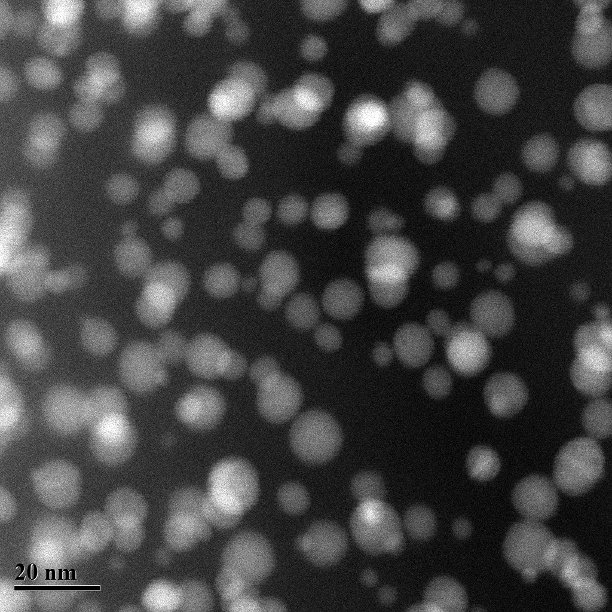
\includegraphics[width=0.5\textwidth]{setup/Au_8008}}
\subfloat[Si nanoparticles.\label{fig_tem_si_np}]{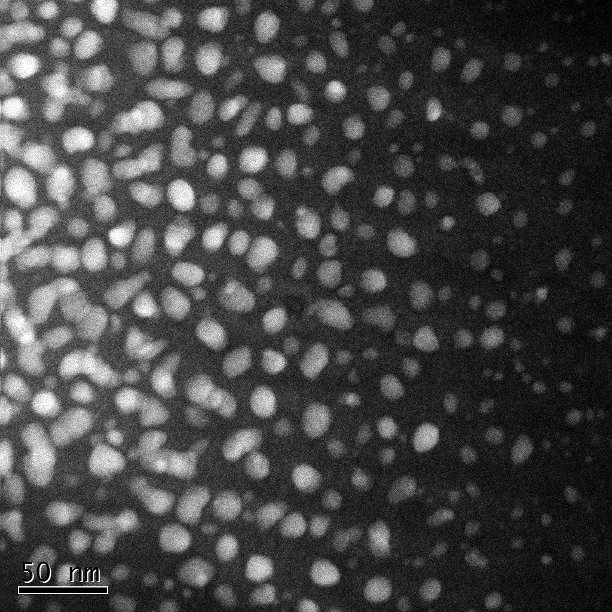
\includegraphics[width=0.5\textwidth]{setup/Si_front_0368}}
\caption{TEM scans for two of the samples.}
\end{figure}

\subsubsection{Reference Glass and Substrate}\label{chap_setup_glass}
In addition to the nanoparticle samples, a piece of the same substrate (Suprasil 300) used to embed the nanoparticles was included as a first reference. A second sample of high quality glass from the Femtosecond Spectroscopy lab was used as a second reference.

%%%%%%%%%%%%%%%%%%%%%%%%%%%%%%%%%%%%%%%%% Lasers %%%%%%%%%%%%%%%%%%%%%%%%%%%%%%%%%%%%%%%%%%%
\subsection{Laser System}\label{chap_setup_laser}
The laser used in this setup is a modular ultrafast system with a fundamental wavelength of 800\,nm. It consists of a Spectra-Physics Spitfire Ti:sapphire amplifier, coupled to a Spectra-Physics Merlin pump laser, and a KMLabs oscillator. Pumping the oscillator is a Spectra-Physics Millenia V. The pump and Ti:sapphire cooling is done via two stationary water chillers. Figure \ref{fig_lasers} is a photograph of the system.

The very large size of the amplifier and oscillator allows for easy modification and adjustment. As with most laser systems, we checked power output on a daily basis and  made the appropriate adjustments to maximize available power.

\begin{figure}[h]
\centering
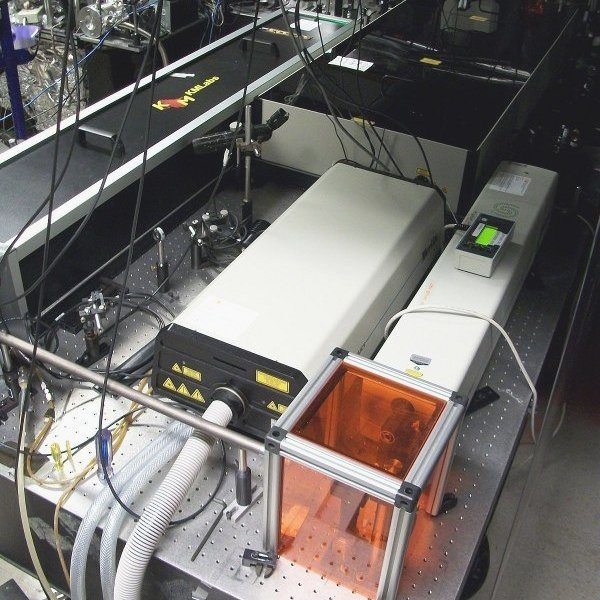
\includegraphics[scale=0.55]{setup/lasers}
\caption[Laser system used in experiment.]{Laser system used in experiment. Clockwise from right: Millenia V, Merlin, KMLabs oscillator, and Spitfire in back.\label{fig_lasers}}
\end{figure}

\subsubsection{Spectra-Physics Millenia V Pump Laser}
This laser pumps the oscillator. It is a diode-pumped, continuous wave, solid-state visible laser that outputs 4.30\,Watts at 532\,nm. It uses a neodymium yttrium vanadate (Nd:YV$\text{O}_{4}$) gain medium that is pumped by two 20\,Watt fiber coupled diode laser bars that are located in the control box. The Nd:YV$\text{O}_{4}$ crystal produces 10\,Watts power at 1064\,nm after amplification. The light is then doubled with a lithium triborate (LBO) crystal to produce close to 5\,Watts.

\subsubsection{KMLabs Ti:sapphire Laser Kit}
The oscillator system is a KMLabs Ti:sapphire Laser Kit. It was designed to be built and alligned by the user and was sold disassembled. It requires close to 4.5\,Watts of 532\,nm pump light in $\text{TEM}_{00}$ mode to produce a 10 - 15\,fs pulse with a bandwidth of 50 - 70\,nm FWHM and an average power of 500\,mW. It has a repetition rate of 76\,MHz. This laser was by far the best behaved during the course of this experiment. Although it needs to be constantly realigned to maximize output, it never stopped working.

\subsubsection{Spectra-Physics Merlin Pump Laser}
This laser acts as the pump for the amplifier. It is a 527\,nm Q-switched pump laser that uses a neodymium-doped yttrium lithium fluoride (Nd:YLF) active medium. The Nd:YLF rod is optically pumped with an arc lamp and is water cooled. The rod emits light at 1053\,nm, which is then doubled by an LBO crystal to 527\,nm. It has a repetition rate of 1\,kHz and produces 10\,mJ of energy per pulse. 

\subsubsection{Spectra-Physics Spitfire Laser Amplifier}
The Spitfire is a regenerative Ti:sapphire amplifier. It uses two gratings for stretching and compressing the pulse, as is normal with CPA systems. The final output is 1.1 Watts with 1 mJ per pulse at 800\,nm with a pulse duration of around 100\,fs.

%%%%%%%%%%%%%%%%%%%%%%%%%%%%%%%%%%%%% NOPA %%%%%%%%%%%%%%%%%%%%%%%%%%%%%%%%%%%%%%%%%%%%%%%%%
\subsection{NOPA at Femtosecond Spectroscopy Lab}

We learned about the concepts behind the NOPA in section \ref{chap_theory_nopa}. This NOPA uses a beta barium borate (BBO) crystals to produce SHG. A sapphire window generates the white light continuum needed to seed the crystal. All the elements in the beam path stretch the pulse temporally -- two large prisms are used to re-compress it back down to an acceptable length.

It is tunable via a delay stage. However, it is not a straightforward matter of adjusting the stage and getting a new wavelength. Some parts of the system need to be realigned after moving the stage even a little.

This NOPA produces pulses that are around 250\,fs in duration with a 1\,kHz repetition rate. Pulse energy is between 3 - 12\,$\mu$J, and can be tuned between 1.6 and 2.4\,eV, or 760 - 515\,nm. Figure \ref{fig_nopa_diagram} depicts a diagram of the setup, while figure \ref{fig_nopa_work} shows the NOPA in action.

\begin{figure}[h]
\centering
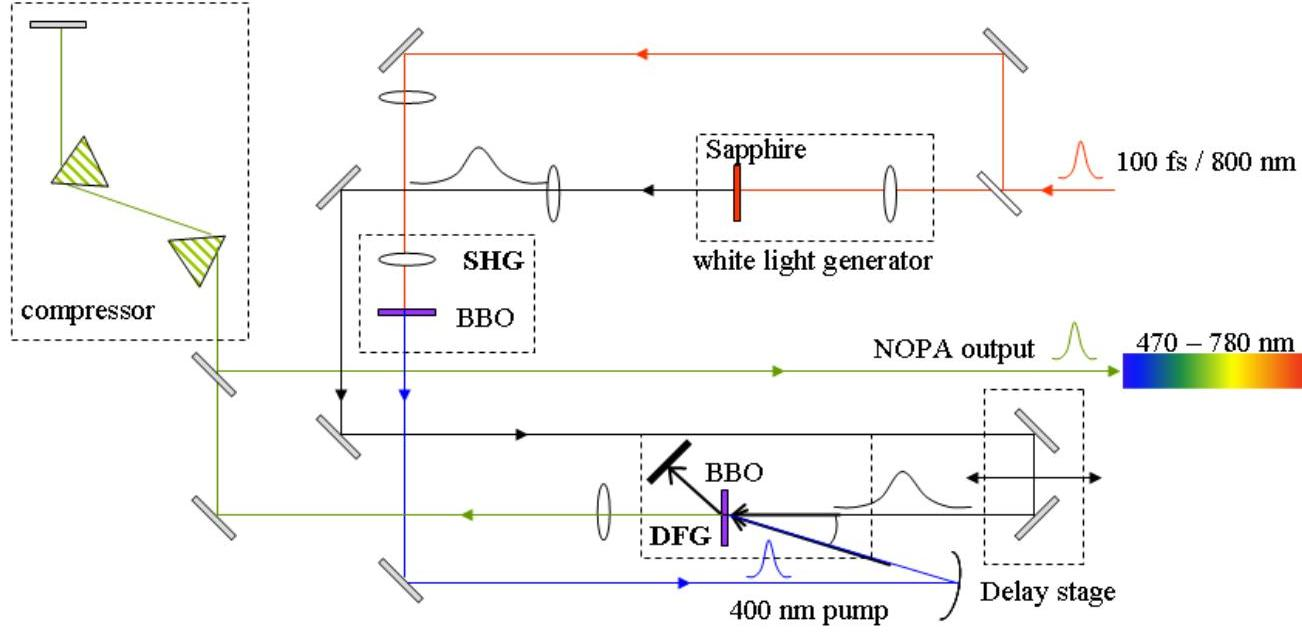
\includegraphics[width=0.95\textwidth]{setup/nopa}
\caption[Diagram of the NOPA at the Femtosecond Spectroscopy Lab.]{Diagram of the NOPA at the Femtosecond Spectroscopy Lab. Image: Adrian Wirth, Junwei Wei.\label{fig_nopa_diagram}}
\end{figure}

\begin{figure}[h]
\centering
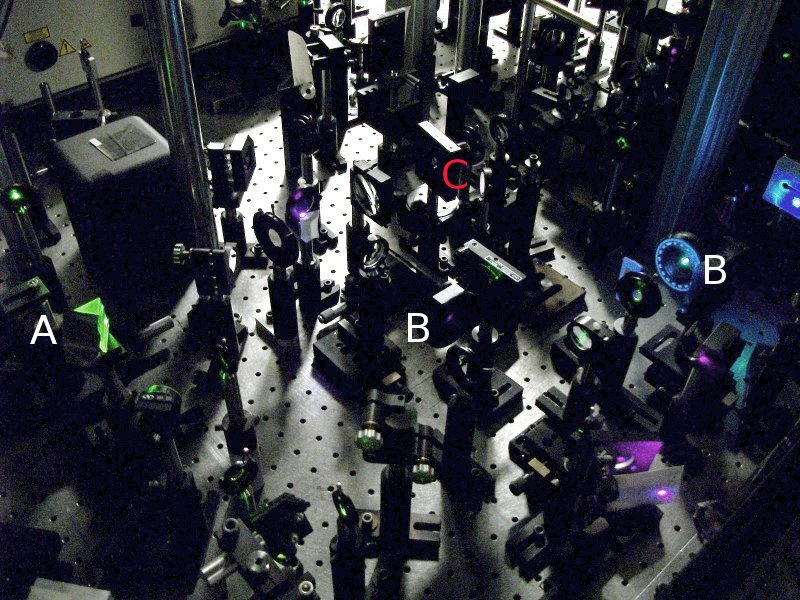
\includegraphics[width=0.95\textwidth]{setup/nopa_pic}
\caption[The NOPA at the Femtosecond Spectroscopy Lab.]{The NOPA at the Femtosecond Spectroscopy Lab. One prism (A), two crystals (B), and the sapphire window (C) can be seen.\label{fig_nopa_work}}
\end{figure}

%%%%%%%%%%%%%%%%%%%%%%%%%%%%%%%%%%%%%% XP2SHG/SFG %%%%%%%%%%%%%%%%%%%%%%%%%%%%%%%%%%%%%%%%%%%
\subsection{The XP2SHG/SFG Elements}
We discussed the foundations for this technique in section \ref{chap_theory_xp2}. The arrangements for both SHG and SFG are very similar; amplified pulses from the laser are used for SHG, and the off-normal beam with the NOPA output is used for SFG. Physically, the setup is a modular optical arrangement placed on two breadboards that snap into place with strong magnets. This allows for easy removal and fast adjustments. Different arrangements can be put in place without totally misaligning the entire setup. The first breadboard contains the delay stage, beam-splitter, and mirrors that allow for fine adjustments and provide the reference signal for the experiment.

\subsubsection{XP2SHG Arrangement}
I will describe the arrangement making reference to the diagram in figure \ref{fig_xp2}. The laser beam is first polarized via a thin film plate polarizer (not pictured), which ensures that the beam is p-polarized. It is then split by a piece of microscope slide (BS1) -- the weak reflection is focused down into a BBO crystal to produce second harmonic light at 400,nm, and is collected by an Oriel spectrometer to use as a quadratic reference.

The main beam is split by a 50/50 beam-splitter (BS2). The straight beam goes into a 1 cm delay stage used as a variable time delay in order to temporally overlap the pulses on the sample. This beam arrives at the sample at normal incidence, so dipolar SHG from the substrate surface is strictly forbidden by selection rules. Lastly, it is focused down via a fixed 50\,mm lens (L3).

The other beam is redirected through a half-wave plate (WP) which polarizes it vertically. It arrives at the sample s-polarized, and initially at an angle $\phi_{0}$ of 20 degrees. Later on we separated the beams further to avoid scattering and increased the angle to 40 degrees. Dipolar SHG is also forbidden from the substrate surface for this beam as long as it is s-polarized. This beam is focused with a 50\,mm lens (L4). There is an optional BBO crystal on a folding arm that can be used to verify spatial and temporal overlapping of the two beams. This crystal cannot be used once the sample is in place. Figure \ref{fig_xp2_assembly} shows the second breadboard containing these elements. Figure \ref{xp2shgdark} depicts how intense the SHG signal is when everything is overlapped properly using the BBO crystal.

\begin{figure}[h]
\centering
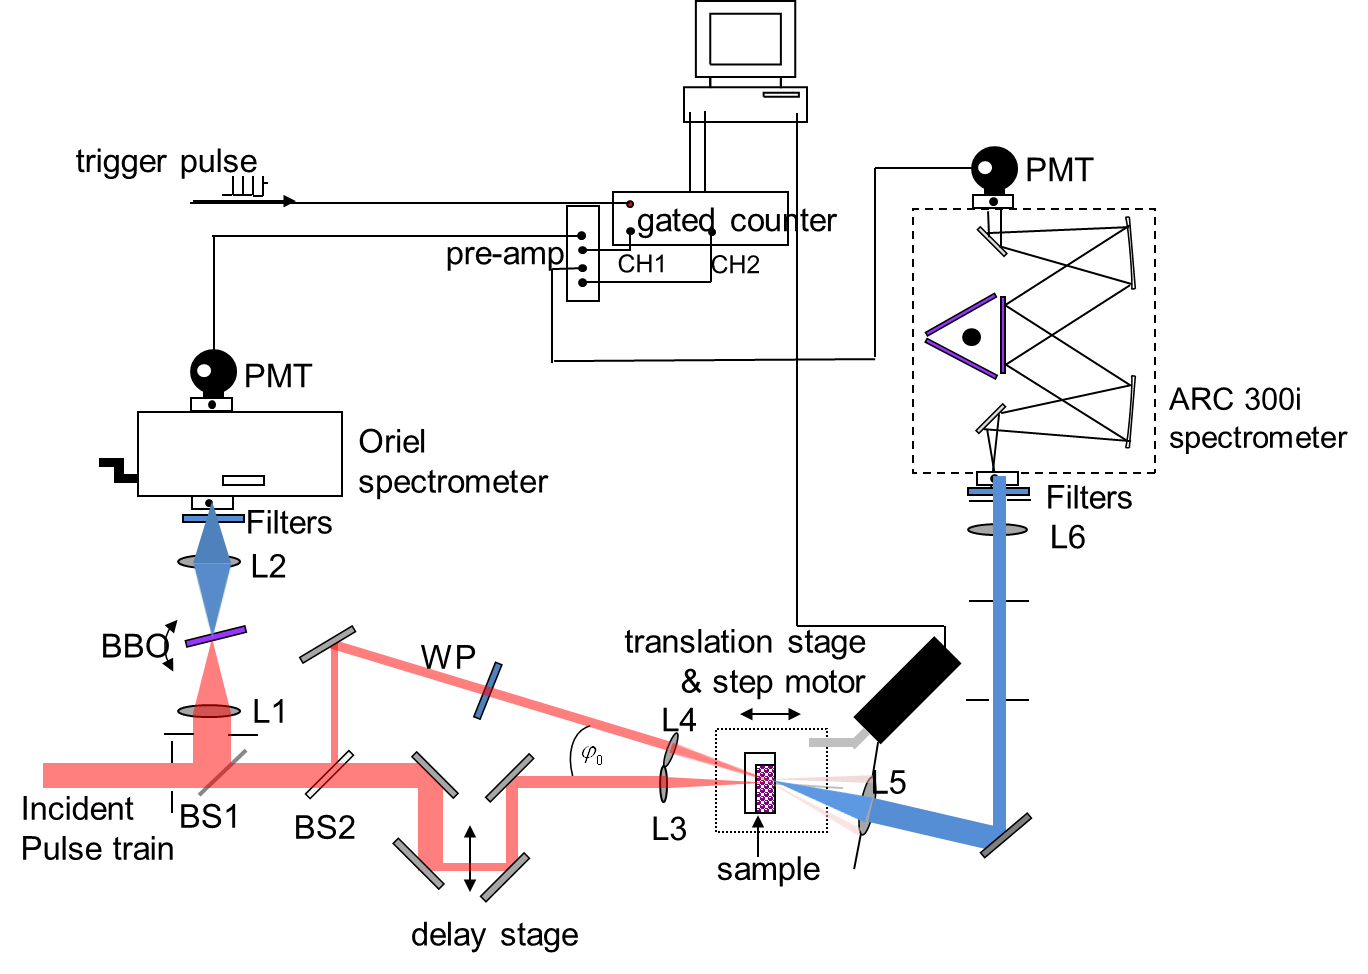
\includegraphics[width=\textwidth]{setup/XP2SHG_setup}
\caption[A diagram of the XP2SHG arrangement.]{A diagram of the XP2SHG arrangement. Image: Junwei Wei.\label{fig_xp2}}
\end{figure}

Finally, the beams are focused down on the sample with an approximate spot size of 250\,$\mu$m. Behind the sample is an iris with a collecting lens (L5). From there, the signal is captured by the ARC 300i monochromator/spectrometer. I will describe these detectors in greater length in section \ref{chap_setup_det}.

The sample holder is built on a linear translation stage. It is controlled by a stepper motor that can be accessed via a computer. This allows us to control the motion of the sample during the experiment; the motion is stopped automatically with the recording of each data point.

\begin{figure}[h]
\centering
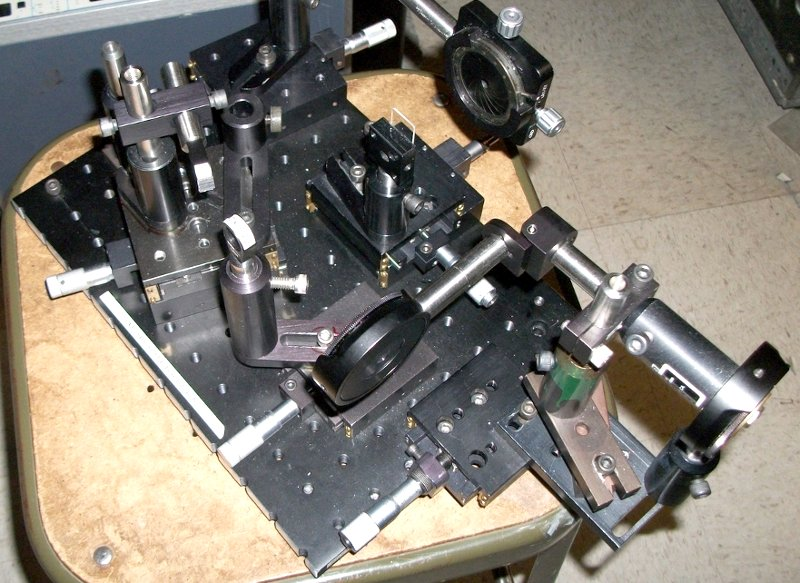
\includegraphics[width=0.86\textwidth]{setup/xp2shg_assembly}
\caption[Second XP2SHG breadboard.]{Second XP2SHG breadboard. Substrate sample in holder and BBO crystal folded away at middle.\label{fig_xp2_assembly}}
\end{figure}

\begin{figure}[h]
\centering
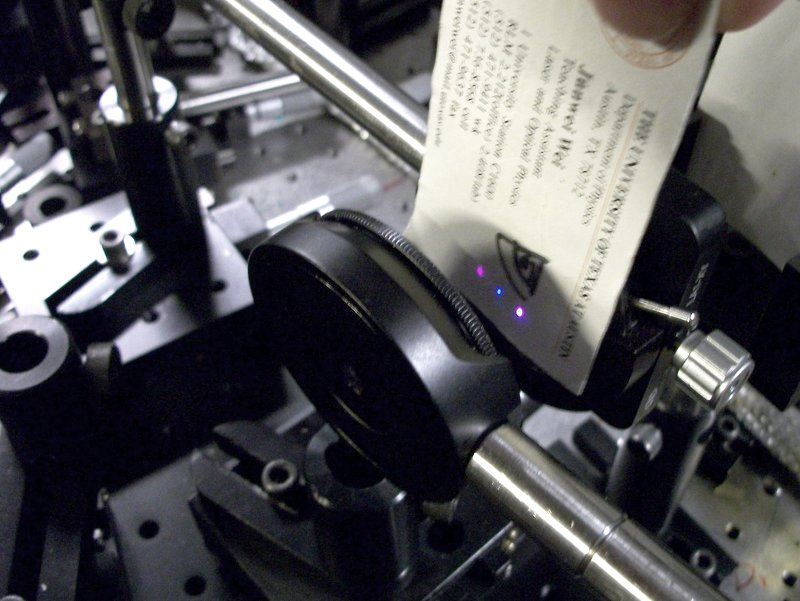
\includegraphics[width=0.86\textwidth]{setup/xp2shgdark}
\caption{XP2SHG with a BBO crystal.\label{xp2shgdark}}
\end{figure}

\subsubsection{XP2SFG Arrangement}
The arrangement remains very similar for SFG measurements. First, we get the NOPA up and running. After it is functioning at maximum efficiency, its output is fed into the XP2SFG path. BS2 is no longer needed, but the output is typically so energetic that it is easier to leave it in and block the redirected beam. In its place, a beam split off from the main amplifier output is used. This beam comes around the entire setup and an extra mirror must be inserted to redirect the new beam into the focusing lens. When set up like this, we used two filter holders (one for each beam) to provide fine attenuation to each. These consisted of various neutral density and color filters (UG5 and OG515).

%%%%%%%%%%%%%%%%%%%%%%%%%%%%%%%%%%%%%%% Detectors %%%%%%%%%%%%%%%%%%%%%%%%%%%%%%%%%%%%%%%%%%
\subsection{Detection System}\label{chap_setup_det}
The detection system captures two sources of light -- the light produced from the sample, and a reference beam that we use to compare with the sample signal. Having the reference is important to correlate fluctuations in the laser output with corresponding fluctuations in the signal output. After we get the data we can normalize the signal data with the reference data to get a more accurate idea of what happened during the run.

The signal beam is captured in a Acton Research Corporation SpectraPro-300i monochromator, with a Hamamatsu R4220 photomultiplier tube (PMT) attached to it (figure \ref{fig_monochromator}). The ARC SpectraPro-300i is a 30\,cm monochromator that allows three grating choices. It is attached to a computer system with proprietary software installed that allows for manual grating and wavelength selection, or automated scans across a range.

The reference beam is captured by an Oriel 77250 monochromator coupled to another Hamamatsu R4220 PMT. The Oriel 77250 is a 12.5\,cm, single grating monochromator that is manually controlled via a hand-crank to turn the grating. It has no software control.

An Ocean Optics fiber spectrometer is sometimes used to determine the wavelength of the signal beam in the NOPA. It is PCI format and located inside a computer. A fiber is connected to it with the other end placed in the optical setup when needed. It is not used for recording data.

\subsubsection{Hamamatsu R4220 PMT}
The Hamamatsu R4220 PMT is a side-on, 28\,mm PMT. It detects in the range of 185 - 710\,nm, with its peak sensitivity at 410\,nm and a quantum efficiency of around 22\% at that wavelength. Although it has a broad sensitivity curve, it has the highest sensitivity and quantum efficiency in the 300 - 450\,nm range. This makes it optimal for detecting SFG and SHG signals which usually are between 300 - 400\,nm. The cut off wavelength is around 750\,nm, so it does not detect the Ti:sapphire fundamental of 800\,nm. It has a built in high voltage power supply that requires 15\,V to function. 

\begin{figure}[h]
\centering
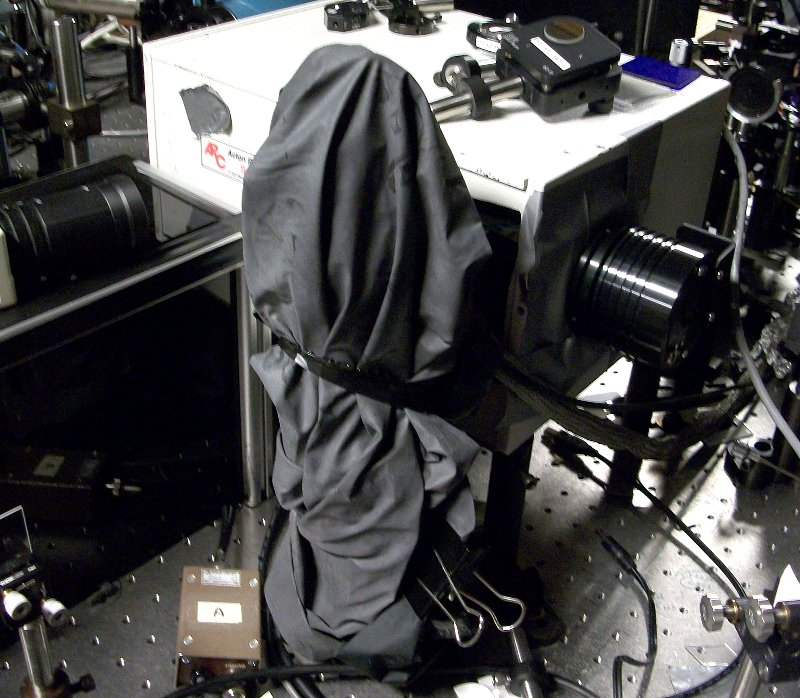
\includegraphics[width=0.9\textwidth]{setup/monochromator}
\caption{ARC SpectraPro-300i Monochromator with shrouded PMT.\label{fig_monochromator}}
\end{figure}

\subsubsection{Electronics}
Several pieces of electronic equipment are needed to control and record the signals from the PMTs. The measurement equipment is primarily manufactured by Stanford Research and is mounted in an Ortec 401A Modular System Bin. Outside of the bin reside the power supply for the PMTs, the Stanford Research SR400 photon counter, a Tektronix 7903 oscilloscope, and the computer used to control and record all data runs. See figure \ref{fig_electronics} for a picture of the setup.

\subsubsection{Equipment in Ortec 401A}
Inside the Ortec 401A is all Stanford Research equipment. The SR240 Fast Preamp is the amplifier used for both PMTs. Each PMT signal gets amplified two times in the SR240. The output of a PMT is connected to the input of one channel, then its output gets connected to the input of a second channel. The final output of each goes either to the SR250 gated integrator, or to the SR400 photon counter. The SR240 is a 350 MHz preamplifier with a gain factor of 5 per channel; this means that the output of each PMT is increased 25 times.

The SR245 is a computer interface that has both serial and GPIB ports to communicate with computers. This module is not in use however, since the computer system has its own PCI GPIB card.

Lastly, the SR250 Gated Integrator. This boxcar integrator is designed for signal recovery and is especially suited for use with fast events. It consists of a gate circuit that is only activated when externally triggered. In this way, the integrator is very useful for signal recovery because integrates and averages during very small windows of time. If the noise floor is relatively high, this can effectively isolate a signal and recover its features over the course of the measurement. The external trigger in our setup is supplied by the laser amplifier. However, since this device integrates and averages, it is no good for extremely small signals like the ones emitted by the samples which would get lost when averaged together. So this device is only used when optimizing and calibrating the setup.

\subsubsection{Stanford Research SR400 Photon Counter}
The SR400 is a dual channel photon counter that offers very sensitive, single photon measurements. It integrates amplifiers, discriminators, gate generators, and counters all in one unit. Each channel has its own set of instrumentation and can count at rates up to 200 MHz. Discriminators allow individual pulses to be filtered out from background noise. 

This piece of equipment was the cornerstone of this entire experiment. Our SHG and SFG signal strength was in the hundreds of photons (per two or three seconds) for our best runs. Only a photon counter, coupled with a very good PMT can read and record such low signals.

\begin{figure}[h]
\centering
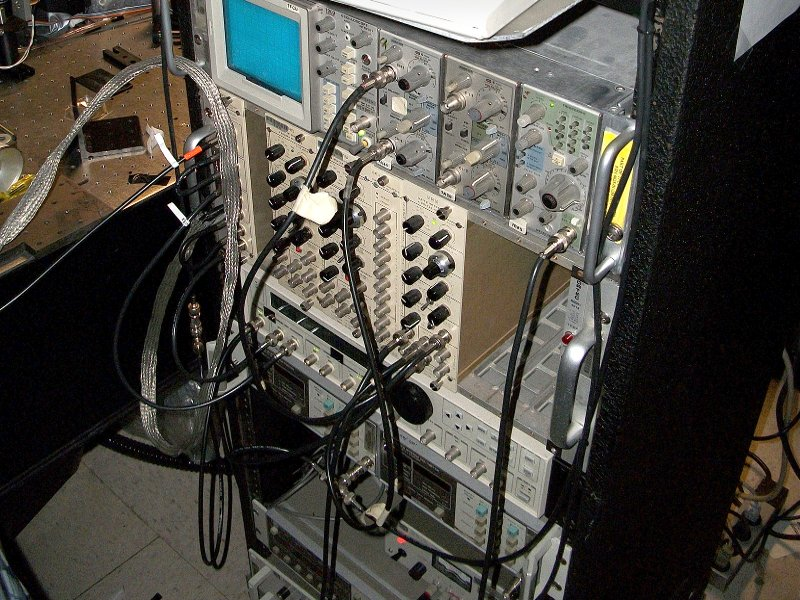
\includegraphics[width=0.9\textwidth]{setup/electronics}
\caption[Electronics for detection equipment.]{Electronics for detection equipment. From bottom device with red light: power supply for PMTs, HP Voltimeter, Stanford Research SR400, Ortec 401A, and Tektronix 7903 oscilloscope. In Ortec rack from left to right: SR240 Fast Preamp, 2 $\times$ SR250 Gated Integrator, SR245 Computer Interface, and SR250.\label{fig_electronics}}
\end{figure}

\subsubsection{Computer System}
The computer system is a standard desktop machine that runs homebrew NI LabVIEW programs under Microsoft Windows 2000. These programs control the movement of the sample holder which is located on a linear stage, and simultaneously record data at each stop. The program most used for this research records the stage position in steps, the SHG/SFG signal, the reference signal, and the ratio of the two. It has its own GPIB interface which is directly connected to the SR400 for data acquisition. This data is stored in a simple text file for later plotting and analysis.

%%%%%%%%%%%%%%%%%%%%%%%%%%%%%%%%%%%%%%%%%%%%%%%    %%%%%%%%%%%%%%%%%%%%%%%%%%%%%%%%%%%%%%%%%%%%%
%%%%%%%%%%%%%%%%%%%%%%%%%%%%%%%%%%%%%%%%%%%% Procedure %%%%%%%%%%%%%%%%%%%%%%%%%%%%%%%%%%%%%%%%%
\section{Procedure}
\subsection{Linear Measurements}
The linear measurements for the samples were taken at the Center for Nano and Molecular Science and Technology in the Nano Fabrication and Testing Facility at UT Austin. The samples underwent linear transmittance analysis in a Varian Cary 500 UV-Vis Spectrometer, and spectroscopic ellipsometry (SE) in the cleanroom using a J.A. Wollam M2000 Spectroscopic Ellipsometer. Thanks go to Junwei Wei for taking these measurements.

\subsection{Adjustments Prior to Running XP2SHG/SFG}

\subsubsection{Optimizing Laser Output}
The first step for the XP2SHG experiment is optimizing the laser output into the optical arrangement. We turn the laser system on and  leave it running for about half an hour to ensure stability. Then, the laser power is measured at the exit aperture using a power meter. The delay times for the Pockels cells are adjusted for maximum output using the same power meter. A mirror is placed in front of the Spitfire output beam reflecting it through a lens that focuses the beam down. A screen shows the resulting nonlinear blotch produced by the plasma being created by the beam. Adjusting the compressor length inside the Spitfire via the motorized adjustment control changes the brightness and color of the blotch; the output of the laser is at its most energetic when at maximum brightness.

\subsubsection{Optimizing Overlaps and SHG/SFG Output}
The signal from the laser or the NOPA arrangement (for SHG or SFG) is introduced into the XP2SHG/SFG optics after the laser system has been set to maximum output. However, a good stable laser signal is not enough to ensure that the XP2SHG setup will work correctly -both beams need to be both spatially and temporally overlapped.

Spatial overlap is usually done by eye. The two beams are placed on a screen located at the focal point of the two lenses and the mirrors are adjusted until both hit the same spot on the screen. This can be verified using a telescope lens arrangement, but this method is rarely used as visual confirmation is good enough. Regardless of SHG or SFG, the two beams must coincide as closely as possible. A business card works as a screen although the NOPA beam in SFG is usually dimmed because the human eye is extremely senstive to green and it appears to overpower the 800 nm beam.

The BBO crystal is then swung into place above the sample holder. It is designed to be at the common focal point of both lenses. Its mount can be rotated to facilitate proper phase-matching conditions. Only proper spatial and temporal overlapping will allow the crystal to produce the SHG/SFG signal. The direction of the output signal is always exactly between the other two beams. See figure \ref{xp2shgdark} for a picture of the BBO output.

At last we come to the question of finding the temporal overlap. Both of the beams consist of trains of pulses that move along the optical path. Pulses from both trains have to coincide at the same time on the sample in order to produce a nonlinear signal. This is adjusted via the delay stage for the normal incidence beam and has to be done if any adjustment is made to the setup that changes the optical path. This includes the introduction of filters or moving any element along the beam line. Once a position is set on the micrometer adjuster, it can typically be referred back to as long as the path has not changed.

In summary, a normal overlap adjustment consists of simultaneously adjusting off beam mirror, the rotation on the crystal, and the delay stage on the beam at normal incidence. If the crystal produces a nonlinear signal, that means that everything is overlapped correctly and the data run can finally start using the desired sample.

\subsubsection{Adjusting the Detector System}
The amplified reference PMT output is connected to the gated integrator which connects to a voltmeter. It displays a voltage reference that is relative to the amplitude of the signal being detected. For SFG, the wavelength of the NOPA signal is measured using the Ocean Optics spectrometer and the grating setting on the monochromator is adjusted via computer to obtain the closest wavelength possible to the signal produced by the sample. The numbers on the voltmeter display increase as the correct wavelength is approached.

Once the proper grating position is selected, we can do any final alignment in the optical setup. Again, looking at the voltmeter allows us to properly adjust any mirror angles, etc. This part is also the appropriate time to select the right filters to use in order to attenuate the beam intensities. If the voltmeter displays a large number ($>$ 1\,V $\approx$ 15\,mJ/cm$^{2}$) we are at risk of damaging the sample. Although the damage threshold is different for all samples, experience has proven that samples of this nature (implanted on fused silica substrates) are safe at these levels.

We then turn the photon counter to check background noise levels. Electrical noise will often seep into the detection line and greatly raises the noise floor. This shows up on the photon counter as hundreds of counts per second. Jostling the electronics rack or placing tin foil on the cabling will often fix the problem. The experiment is ready to run as soon as the photon count remains close to zero when restarting the counter.

Lastly, the computer is turned on and Labview is started. The custom program interfaces are all labview programs that are automatically set up to communicate with both the photon counter and the translation stage under the sample. The program used in this experiment presents a table that updates itself with each value measured for both the reference and sample signals. It allows the user to select the direction of the platform, the amount of steps to travel, and the starting and stopping points. Unfortunately the platform and stepper motor are very unsophisticated and have no means of relaying back their absolute position data. This means that the stage has to be manually set in the starting position after each run. As a consequence of this, the starting point is never the same between runs. All position data captured by this program is therefore only valid for that particular run. Any comparisons made between runs ignore the individual steps traveled.

\subsection{First Experiments - XP2SHG Data Runs}\label{chap_setup_proc_shg}
We first measured the reference glass and substrate. Both of these behaved properly and we moved on to the nanoparticle samples. Here our troubles began. We immediately obtained a very strong signal that turned out to be white light generation, indicating that the incoming intensity was much too strong. Upon attenuating with filters and redoing overlaps, we obtained a very weak and noisy signal from the samples.

Little usable data was obtained even after playing around with the signal intensity and beam size. What interpretable data we did get was not distinguishable from the substrate contribution. We checked all three samples and the same thing was happening with each. Besides all this, there was so much input beam scattering coming from the particles that they obscured any SHG signal. We also realized that often we were actually seeing single beam SHG instead of two beam SHG. It became impossible to tell if what we were measuring was actually two beam from the nanoparticles, some contribution from the substrate, scattering or other noise, or even single beam SHG. Closing irises down improved the signal but not enough to provide usable data.

At this point the samples were taken to clean room for ellipsometry. It was at this point that we noticed that the substrate was in poor condition on every sample. This would account for scattering and the poor interaction between the incoming light and the nanoparticles. We needed a way to reduce scattering as much as possible and reduce any signal emitted from the substrate. 

\subsection{Second Experiments - XP2SFG Data Runs}\label{chap_setup_proc_sfg}
Prof. Downer gave us valuable input on the problem. He suggested that we should switch to SFG, and separate the beams even further. With SFG, all three beams would be of different wavelengths: the fundamental 800 nm off-angle beam, the normal incidence NOPA beam, and the final SF signal from the sample. The NOPA operates most efficiently around 510 - 550 nm which is coincidentally the same range for the plasmon resonance of gold. The separation of the beams would allow us to easily block them on the other side of the sample with an iris without losing any of the desired signal. 
 
Once all that work was done we were ready to try out the samples. The modifications had the intended effect of reducing scattering -- closing the iris behind the sample blocked out most of the scattered light from the input beams. The SFG signal was also clearly different in wavelength than the other two as measured by scanning the monochromator while taking counts at the same time. We were able to filter out the different wavelengths at the detector and confirmed that we were seeing SFG. However, it was not any clearer if what we were seeing was coming from the nanoparticles or the substrate.

One of the unfortunate side effects of switching to SFG was a significant signal decrease. The 800 nm beam was also causing considerable white light generation from the sample. Attenuating it would produce no signal at all. This left little room to obtain a usable signal from the sample.

\section{Summary}
This chapter offers a brief overview of the different equipment used as well as the general procedure followed for this experiment. In chapter \ref{chap_results} I will present the data obtained with appropriate analysis based on the the concepts we reviewed in chapter \ref{chap_theory}.

\chapter{Results and Analysis}\label{chap_results}
\minitoc

%%%%%%%%%%%%%%%%%%%%%%%%%%%%%%%%%% Intro %%%%%%%%%%%%%%%%%%%%%%%%%%%%%%%%%%%%%%%
The results obtained here were taken over the course of a month at the Femtosecond Spectroscopy Laboratory. All figures unless mentioned otherwise were generated by me.

Original datasets were recorded as plain text files with whitespace separated columns as depicted in figure \ref{fig_datafile}. Column two is the relative position of the stage (in steps), column three is the signal count, column four is the reference count, and column five is the ratio between the two. Column one is always null.

\begin{figure}[h]
\begin{Verbatim}[frame=single,fontfamily=courier,fontsize=\small]
0  2700  38.000   3656.000  0.010
0  2750  51.000   3618.000  0.014
0  2800  48.000   3575.000  0.013
0  2850  53.000   3624.000  0.015
0  2900  39.000   3706.000  0.011
0  2950  37.000   3431.000  0.011
0  3000  43.000   3556.000  0.012
0  3050  70.000   3360.000  0.021
0  3100  167.000  3459.000  0.048
0  3150  243.000  3243.000  0.075
0  3200  317.000  3387.000  0.094
0  3250  230.000  3158.000  0.073
0  3300  151.000  3173.000  0.048
0  3350  80.000   3339.000  0.024
\end{Verbatim}
\caption[Example data file.]{Example data file, from left to right: null column, position, signal counts, reference counts, ratio between the two.\label{fig_datafile}}
\end{figure}

Most of the figures in this chapter were created by plotting the ratio of the signals (normalized counts) against the position of the platform. The position of the platform is in steps and was multiplied by 0.625 to yield micrometers, the unit used in the figures. 

%%%%%%%%%%%%%%%%%%%%%%%%%%%%%%%%%% Linear Transmission %%%%%%%%%%%%%%%%%%%%%%%%%%%%%%%%%%%%%%%
\section{Linear Transmission}
Figure \ref{fig_transmission} shows the transmission curves for all samples. Substrate absorption dominates in the 200 - 350 nm range. The spectrophotometer switches lamps at 350 nm which accounts for the abrupt drop in all samples. The two gold samples demonstrate plasmon resonance around 530 nm that coincides with a drop in transmittance. This result coincides with literature \cite{schaadt2005enhanced, lin2005one}.

Strangely, the transmission curve for the silicon nanoparticles is almost completely flat. When physically compared with the samples described in \cite{PhysRevB.84.165316}, this sample appears to be a much darker gray color. Likewise, the transmission spectra of those samples do present an absorption region while this sample does not.

\begin{figure}[h]
\centering
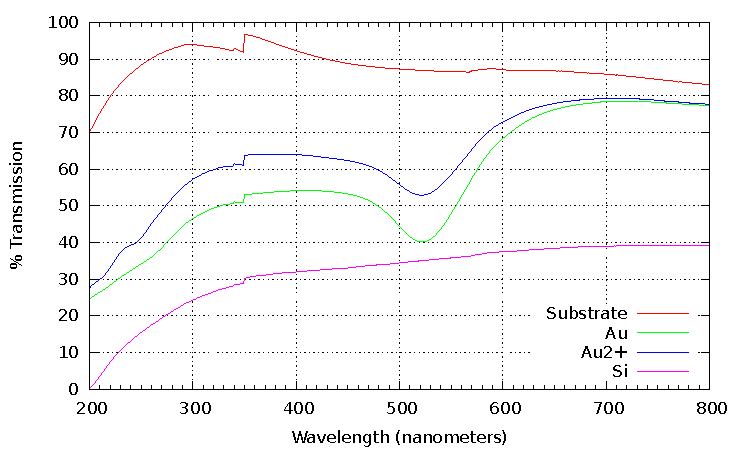
\includegraphics[width=\textwidth]{results/linear_transmission}
\caption{Transmission curves from the three samples and substrate.\label{fig_transmission}}
\end{figure}

%%%%%%%%%%%%%%%%%%%%%%%%%%%%%%%%%% Reference Samples %%%%%%%%%%%%%%%%%%%%%%%%%%%%%%%%%%%%%
\section{Reference Glass and Substrate}
Initial measurements were taken on the glass and substrate samples mentioned in section \ref{chap_setup_glass}. Both glass and substrate present typical behavior when compared to previous measurements taken by the Femtosecond Spectroscopy group.

\subsection{Ellipsometry}
The ellipsometric results shown in figure \ref{fig_sub_ellip} for the substrate are consistent with the data in \cite{PhysRevB.84.165316}. The graphs depict the polarization change represented as an amplitude ratio, $\Psi$, and and the phase difference, $\Delta$. These were the clearest results for this measurement of the four different samples. 

\begin{figure}[h]
  \centering
  \subfloat[Graph for $\Psi$.\label{fig_sub_ellip_1}]{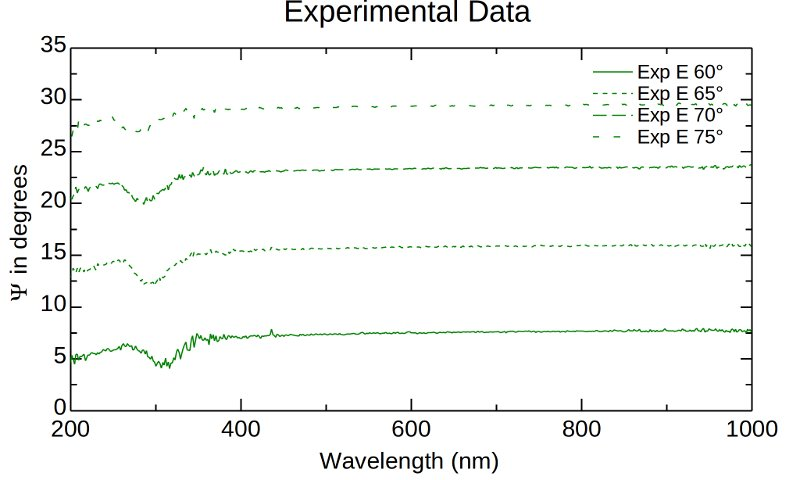
\includegraphics[width=0.5\textwidth]{results/sub_ellipsometry_1}}  
  \subfloat[Graph for $\Delta$.\label{fig_sub_ellip_2}]{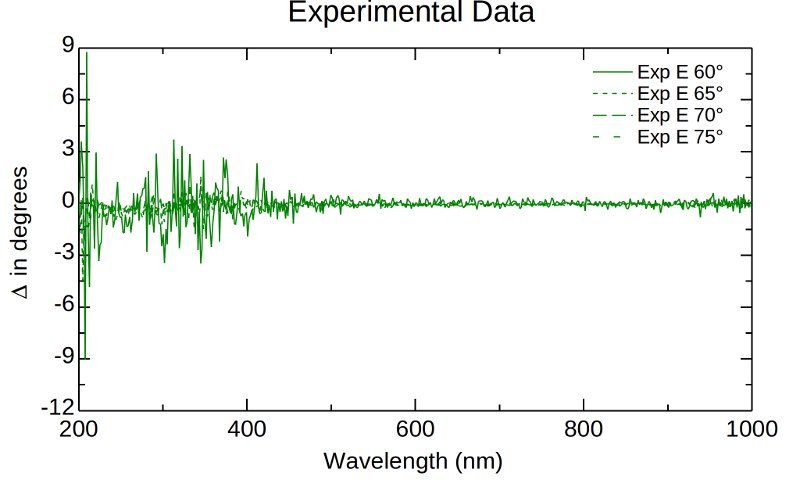
\includegraphics[width=0.5\textwidth]{results/sub_ellipsometry_2}}
  \caption[Substrate ellipsometry.]{Substrate ellipsometry. Graphs courtesy of Junwei Wei.}
  \label{fig_sub_ellip}
\end{figure}

\subsection{XP2SHG and XP2SFG}\label{chap_results_sub_shg}
Figures \ref{fig_glass_shg} and \ref{fig_glass_sfg} both show two distinguishable peaks for the glass reference sample in both SHG and SFG configurations. One peak corresponds to the two beam spots coinciding on the front surface, then on the back and are due to the interference between fields at both surfaces and phase mismatching \cite{sun2005nonresonant}. These peaks are very similar since this sample has no nanoparticles on it. 

\begin{figure}[h]
\centering
\subfloat[XP2SHG signal.\label{fig_glass_shg}]{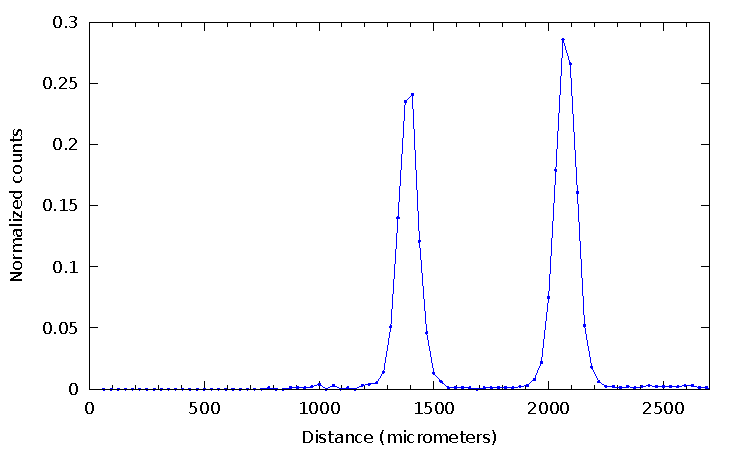
\includegraphics[width=0.5\textwidth]{results/glass_shg}}
\subfloat[XP2SFG signal from 550 and 800 nm beams.\label{fig_glass_sfg}]{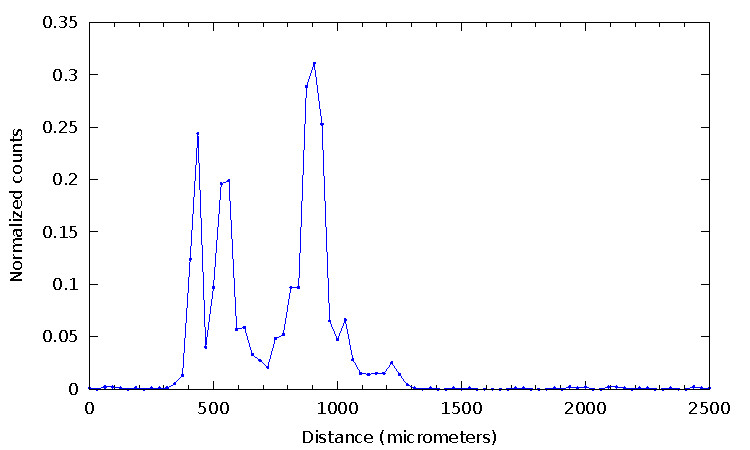
\includegraphics[width=0.5\textwidth]{results/glass_sfg_550+800}}
\caption{SHG and SFG Signals from reference glass.}
\end{figure}

The misshapen first peak of figure \ref{fig_glass_sfg} is due to the difficulty of properly filtering both beams in SFG. Filtering SHG is easier because there are only two wavelengths involved: the fundamental and the signal. There are three in SFG -- the fundamental, the idler, and the signal. Filtering the SFG setup requires at least two distinct filters, one for the 800 nm fundamental and one for the 550 nm idler. This is why both peaks appear to be broader than in figure \ref{fig_glass_shg}, and also accounts for the discrepancy in the sample width as can be measured by the distance between peaks. The real sample width is closer to figure \ref{fig_glass_shg}, at around 700 micrometers.

The substrate shows very similar peaks, as we can see in figures \ref{fig_sub_sfg1} and \ref{fig_sub_sfg2}. Two peaks are clearly resolved when the NOPA wavelength is at 520 nm. The 550 nm beam is more energetic, which explains the additional signal in between the peaks in figure \ref{fig_sub_sfg2}. This signal is emitted from the bulk material and is due to white light generation. Both figures clearly depict the sample width to be around 500 micrometers in thickness. All these observations are consistent with the literature reviewed in section \ref{chap_theory_xp2}.

\begin{figure}[h]
\centering
\subfloat[XP2SFG signal from 520 and 800 nm.\label{fig_sub_sfg1}]{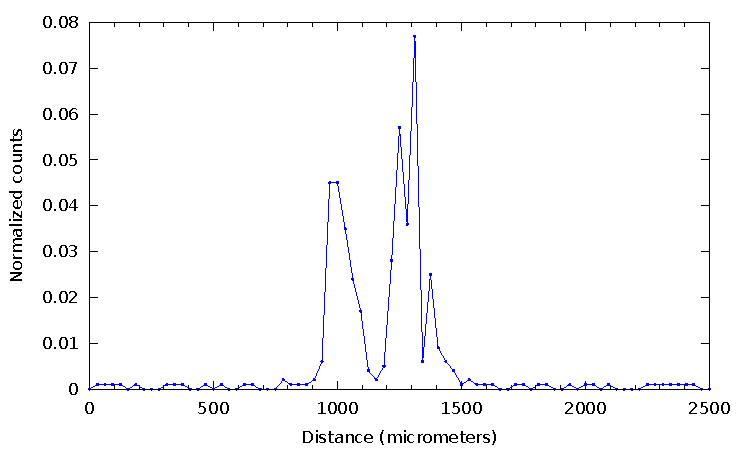
\includegraphics[width=0.5\textwidth]{results/sub_sfg_520+800}}
\subfloat[XP2SFG signal from 550 and 800 nm.\label{fig_sub_sfg2}]{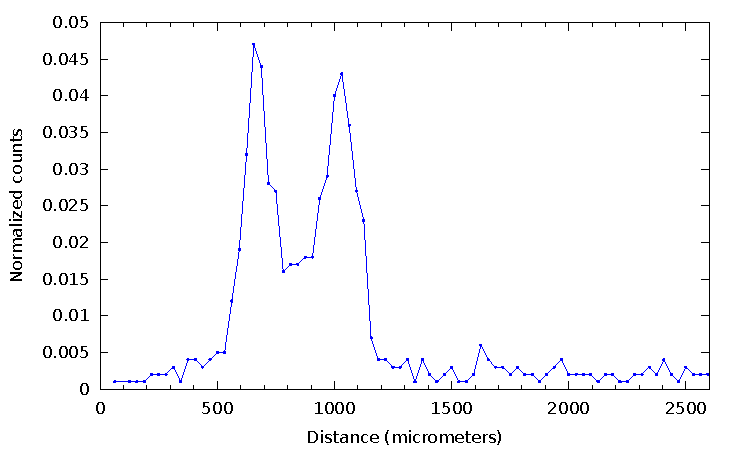
\includegraphics[width=0.5\textwidth]{results/sub_sfg_550+800}}
\caption{SHG and SFG Signals from substrate.}
\end{figure}


%%%%%%%%%%%%%%%%%%%%%%%%%%%%%%%%%% Gold Samples %%%%%%%%%%%%%%%%%%%%%%%%%%%%%%%%%%%%%
\section{Gold Nanoparticles}
The gold nanoparticles were previously described in section \ref{chap_setup_gold}. They underwent the same measurements as the reference samples. Unfortunately these samples present considerable wear and tear that can easily seen with the naked eye. Scratches and other imperfections mar the surface. These imperfections cause a significant amount of scattering. This problem persisted throughout the entire experiment and led to the significant setup change I mentioned at the end of chapter \ref{chap_setup}.

\subsection{Ellipsometry}
Ellipsometric measurements where taken for the gold nanoparticles in the same way as the reference samples. Both sides were analyzed for completeness since it is not always apparent which side has the nanoparticles.

Data from ellipsometry cannot be directly interpreted -- a model must be constructed that fits the data and in the process determines several optical constants, the film thickness, and characteristics of surface. However, the raw data almost always produces well defined curves. The data obtained here is both noisy and unclear. What little distinguishable features that figures \ref{fig_au_ellip_front_1} and \ref{fig_au_ellip_back_1} have are identical to those of the substrate as seen in figure \ref{fig_sub_ellip_1}.

Junwei Wei speculated that the scattering problem is the most likely reason for the unreadable ellipsometry data. Most literature on ellipsometry talk about opaque samples -- these samples are transparent and have a much smaller signal by reflection. He concluded that the data produced here would not yield any relevant results if used with the modeling algorithms.

\begin{figure}[h]
  \centering
  \subfloat[Graph for $\Psi$.]{\label{fig_au_ellip_front_1}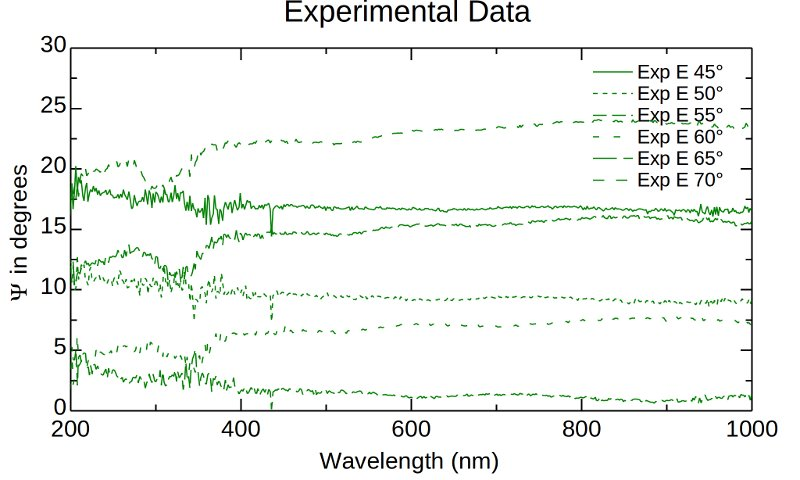
\includegraphics[width=0.5\textwidth]{results/au_ellipsometry_front_1}}  
  \subfloat[Graph for $\Delta$.]{\label{fig_au_ellip_front_2}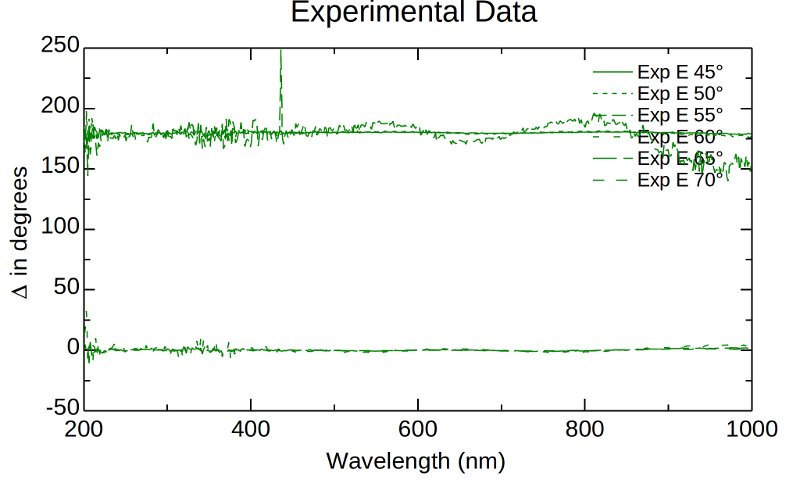
\includegraphics[width=0.5\textwidth]{results/au_ellipsometry_front_2}}
  \caption[Au ellipsometry, front side.]{Au ellipsometry, front side. Graphs courtesy of Junwei Wei.\label{fig_au_ellip_front}}
\end{figure}

\begin{figure}[h]
  \centering
  \subfloat[Graph for $\Psi$.]{\label{fig_au_ellip_back_1}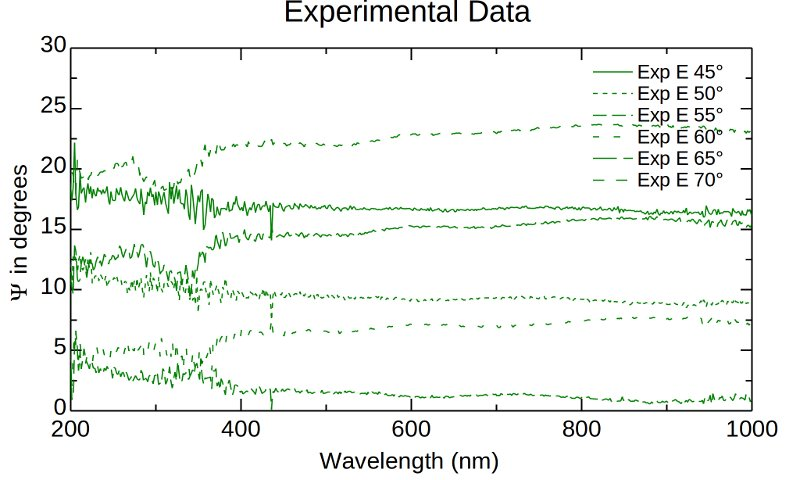
\includegraphics[width=0.5\textwidth]{results/au_ellipsometry_back_1}}  
  \subfloat[Graph for $\Delta$.]{\label{fig_au_ellip_back_2}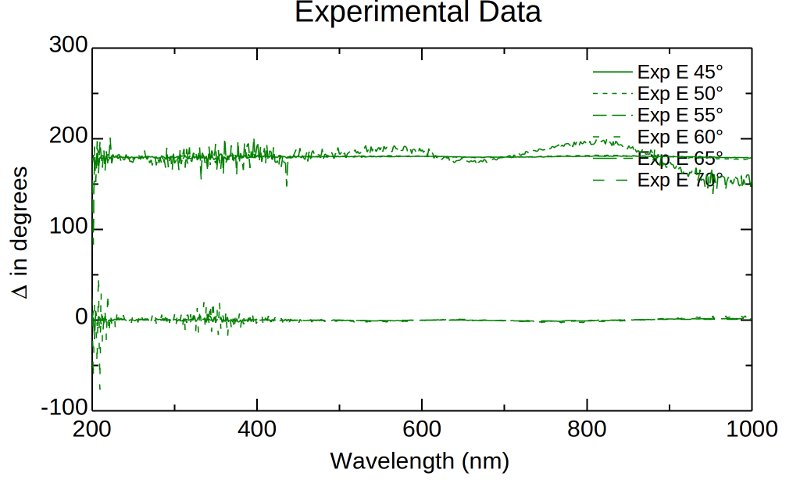
\includegraphics[width=0.5\textwidth]{results/au_ellipsometry_back_2}}
  \caption[Au ellipsometry, reverse side.]{Au ellipsometry, reverse side. Graphs courtesy of Junwei Wei.\label{fig_au_ellip_back}}
\end{figure}

The ellipsometry data for the ionic gold sample (figure \ref{fig_au2+_ellip}) is virtually identical to the others.

\begin{figure}[h]
  \centering
  \subfloat[Graph for $\Psi$.]{\label{fig_au2+_ellip_1}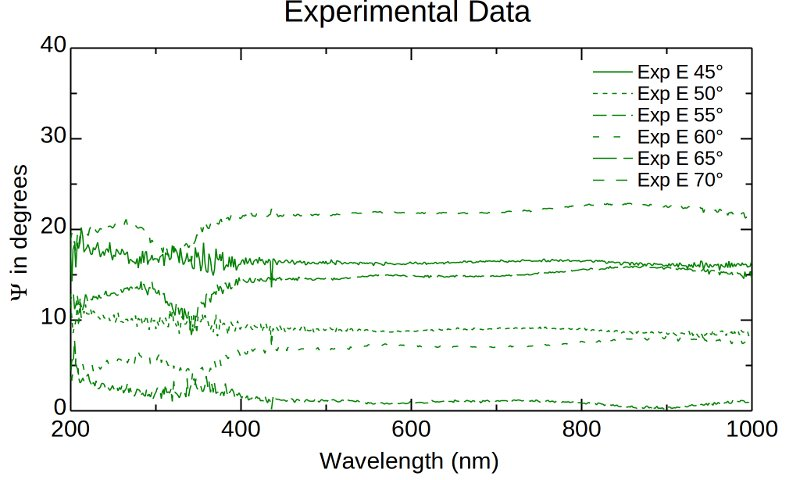
\includegraphics[width=0.5\textwidth]{results/au2+_ellipsometry_1}}  
  \subfloat[Graph for $\Delta$.]{\label{fig_au2+_ellip_2}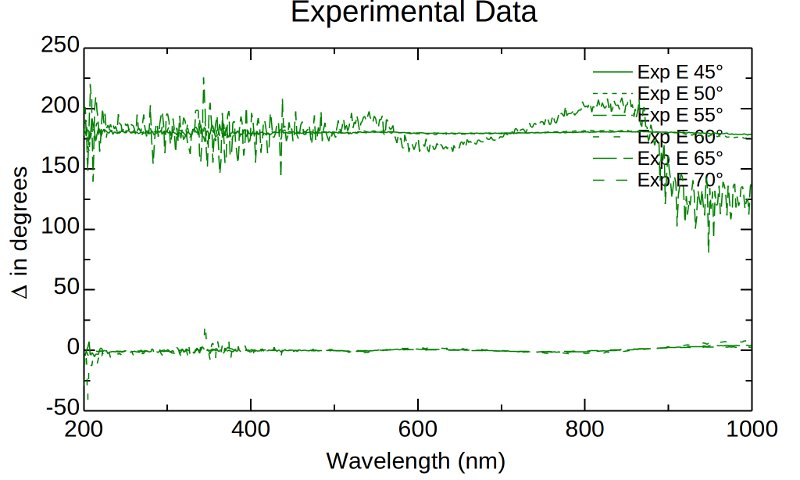
\includegraphics[width=0.5\textwidth]{results/au2+_ellipsometry_2}}
  \caption[Au$^{2+}$ ellipsometry.]{Au$^{2+}$ ellipsometry. Graphs courtesy of Junwei Wei.\label{fig_au2+_ellip}}
\end{figure}

Zhang et al. \cite{zhang2003spectroscopic} detail similar measurements on thin films of gold nanoparticles. Their results show very distinct curves with a clear absorption region. The samples in that article have an absorption band slightly higher than these, centered around 580 nm. These measurements are very noisy compared to the curves depicted there.

\subsection{Filter Tests}
The first thing that is needed is confirmation that the samples can produce a strong second-order signal. A quick filter test is the easiest way to confirm this. The monochromator is scanned across most of the PMT range and the counts are recorded. For figure \ref{fig_filter_no}, we removed all filters from the detectors and blocked the 800 nm beam. Two very prominent peaks corresponding to SHG signal produced in the sample and NOPA were detected with very high intensities. The broadness of the SHG peak (left) is most likely due to white light generation in the crystal for these high intensities.

\begin{figure}[h]
\centering
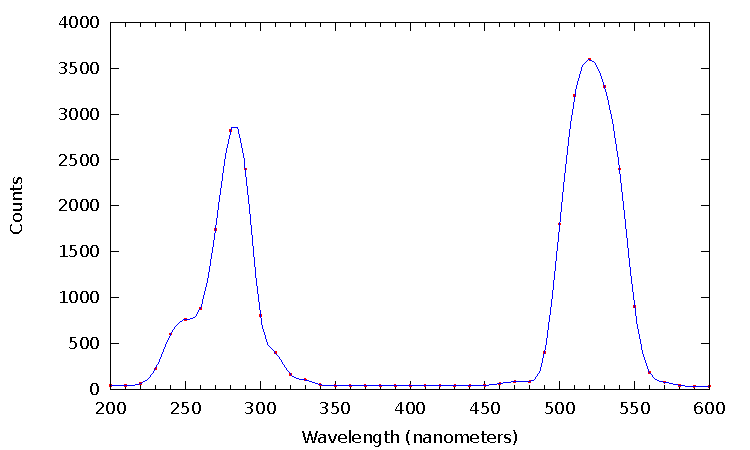
\includegraphics[width=0.875\textwidth]{results/au_nofilter}
\caption{Spectrum from gold sample, no filters.\label{fig_filter_no}}
\end{figure}

We then placed different filters in front of the sample detector. The UG5 filter blocks most light in the 500 - 600 nm range. Placing two in front of the detector block out most of the NOPA signal, as seen in figure \ref{fig_filter_half}. We placed an additional OG515 filter for figure \ref{fig_filter_all}, which blocks out everything below 500 nm and yields only noise. This basic test demonstrates that the sample is indeed capable of producing single beam SHG.

\begin{figure}[h]
\centering
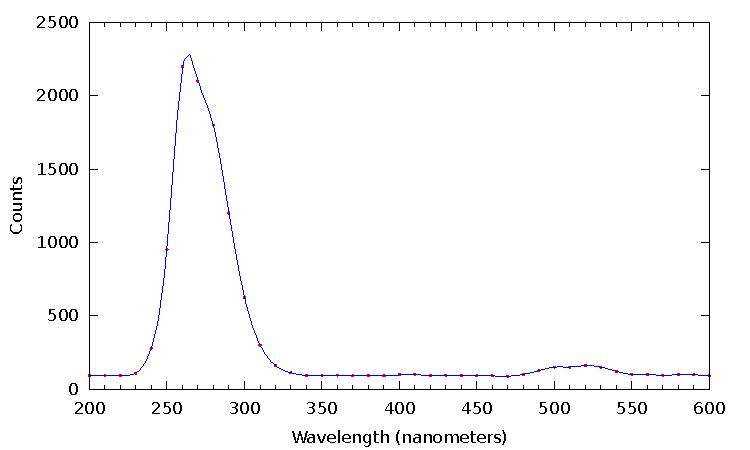
\includegraphics[width=0.875\textwidth]{results/au_ug5+ug5_2}
\caption[Spectrum from gold sample, with filters.]{Spectrum from gold sample, two UG5 filters.\label{fig_filter_half}}
\end{figure}

\begin{figure}[H]
\centering
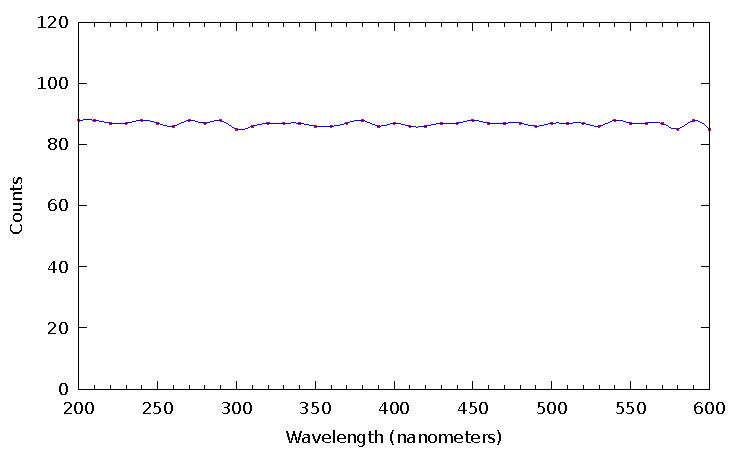
\includegraphics[width=0.875\textwidth]{results/au_og515+ug5+ug5}
\caption[Spectrum from gold sample, with more filters.]{Spectrum from gold sample, two UG5 and one OG515 filters.\label{fig_filter_all}}
\end{figure}

\subsection{XP2SHG Measurements}
Figure \ref{fig_au_shg_narrow} depicts two very well resolved peaks for the Au sample. A higher intensity peak before a lower one means that the nanoparticles were facing the incoming beams in the entrance position. This pattern occurs because the SHG signal is strongest at the nanoparticle surface; for entrance position, the nanoparticles produce SHG first. That signal goes through the remaining glass and is detected. The sample continues to move and SHG is produced on the unimplanted surface, but at a smaller intensity.

A big problem arises when comparing with the substrate data -- how can we distinguish the substrate from the nanoparticles? At first glance, both figures \ref{fig_au_shg_narrow} and \ref{fig_glass_shg} share similarities. We learned that other groups solved this problem (section \ref{chap_theory_xp2}) by taking three separate Z-scans. Naturally, we needed to take data from the samples at both entrance and exit positions.

\begin{figure}[h]
\centering
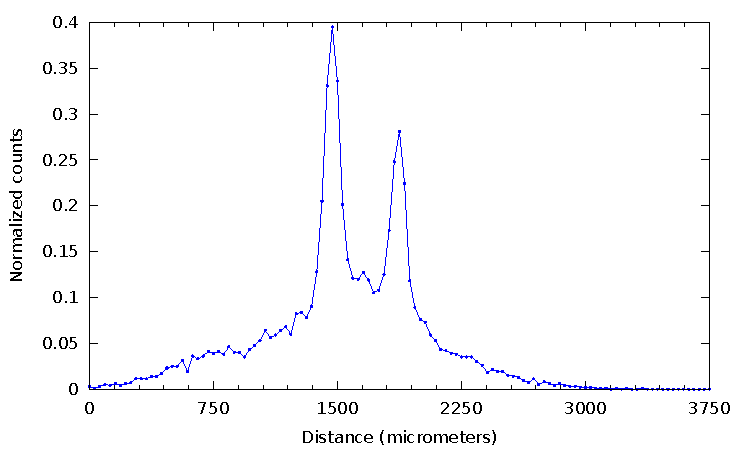
\includegraphics[width=0.9\textwidth]{results/au_shg_narrow}
\caption[Resolved XP2SHG peaks.]{Resolved XP2SHG peaks for gold nanoparticles. Entry side.\label{fig_au_shg_narrow}}
\end{figure}

Figure \ref{fig_au_shg_whitelight} shows the sample in the exit position, with the nanoparticles facing the detector. The order of the peaks is reversed from figure \ref{fig_au_shg_narrow}. For this case, the SHG signal produced by the nanoparticles is free to travel straight to the detector without crossing the substrate. This figure also demonstrates what happens when input intensity is increased slightly. The idea was that increasing the incoming beam would cause a stronger SHG emission from the nanoparticles; instead, white light generation was observed. This is observed in the elongated bump towards the right side of the graph which corresponds to outside the second surface of the sample. Even though the beams were no longer spatially overlapped inside or on the surface of the sample, their intensity was still sufficiently strong to create white light -- perhaps also an indication of some single beam SHG.

\begin{figure}[h]
\centering
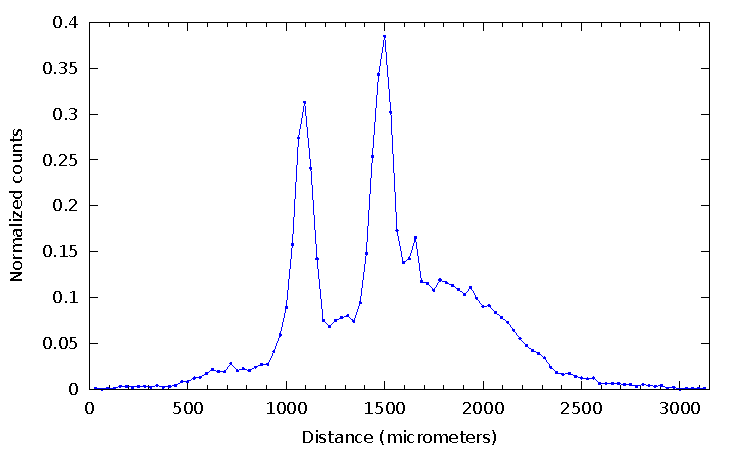
\includegraphics[width=0.85\textwidth]{results/au_shg_whitelight}
\caption[White light generation, gold sample.]{White light generation in gold sample, exit position. Note how counts do not go to zero even when the overlapped beams are outside the sample.\label{fig_au_shg_whitelight}}
\end{figure}

\begin{figure}[H]
\centering
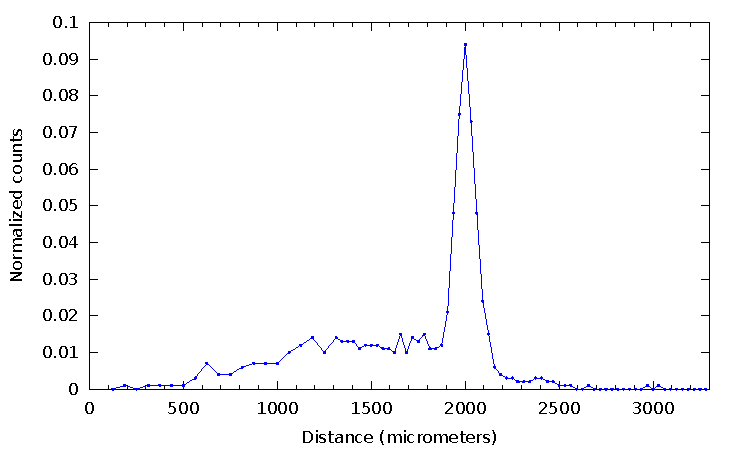
\includegraphics[width=0.85\textwidth]{results/au_shg_best}
\caption{Weaker XP2SHG signal, gold sample.\label{fig_au_shg_best}}
\end{figure}

Lowering the input intensity presented it own share of problems. Figure \ref{fig_au_shg_best} shows SHG emission using one tenth of the previous intensity. The obvious difference is that it lacks an entire peak (also note scale). However, this figure is probably the best data run for the SHG setup; although it lacks a peak, the fact that it was able to radiate at the low intensities is a good case for only nanoparticle contribution without the substrate.

It is easy to read from the previous figures that the sample width is around 500 micrometers, confirming the observation in section \ref{chap_results_sub_shg}.

\subsection{XP2SFG Measurements}
Once the setup had been switched from XP2SHG to XP2SFG, we tested the sample again. Figure \ref{fig_au_sfg_best} represents the best SFG data run with the gold sample. Again, it is impossible to distinguish the substrate contribution from the nanoparticles.

SFG measurements for the gold samples were very inconsistent compared to SHG even though the setup had been properly tested. Figure \ref{fig_sfg_au2+} is a clear example of this. A very noisy signal is present even at relatively high intensities. The two peaks can no longer be resolved.

\begin{figure}[h]
\centering
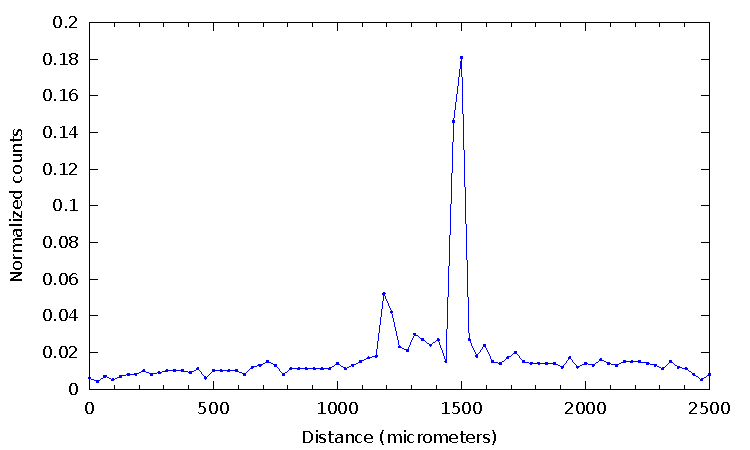
\includegraphics[width=\textwidth]{results/au_sfg_550+800_best}
\caption{Best results for gold sample with XP2SFG setup.\label{fig_au_sfg_best}}
\end{figure}

Scattering was still present even with SFG and an increased beam angle. Most of the data for SFG produced graphs similar to \ref{fig_au_sfg_whitelight}. There is clearly only white light emission with no distinguishable features. This figure in particular was taken with similar input intensities as figure \ref{fig_au_sfg_best} but does not have a similar shape at all.

\begin{figure}[h]
\centering
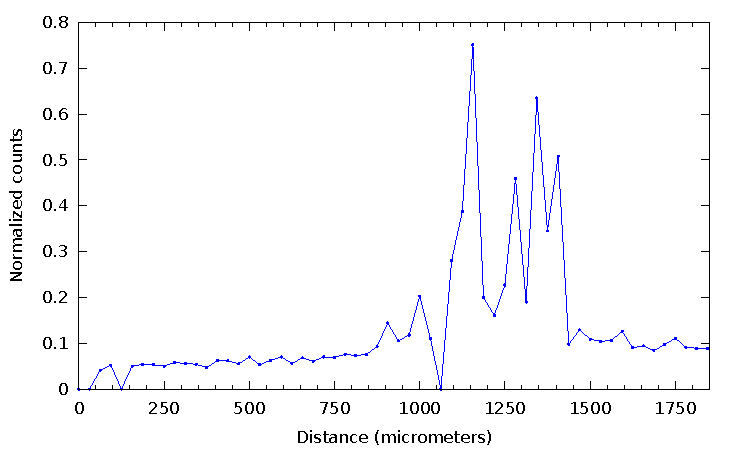
\includegraphics[width=0.9\textwidth]{results/au2+_sfg_520+800}
\caption[Noisy XP2SFG signal for Au$^{2+}$ sample.]{Very noisy XP2SFG signal for Au$^{2+}$ sample. Possible white light emission.\label{fig_sfg_au2+}}
\end{figure}

\subsection{Analysis}
Results where ambiguous at best. The bad physical condition of the samples led to the scattering problem that we never fully resolved. It still presented a problem even after increasing the beam angle and switching from the XP2SHG to the XP2SFG configuration. Shutting down all irises did alleviate the problem, but not enough to be able to present unequivocal data.

Using the 550 nm beam to match the plasmon resonance of the sample became problematic because single beam SHG started to occur, regardless of being in the cross beam geometry.

\begin{figure}[h]
\centering
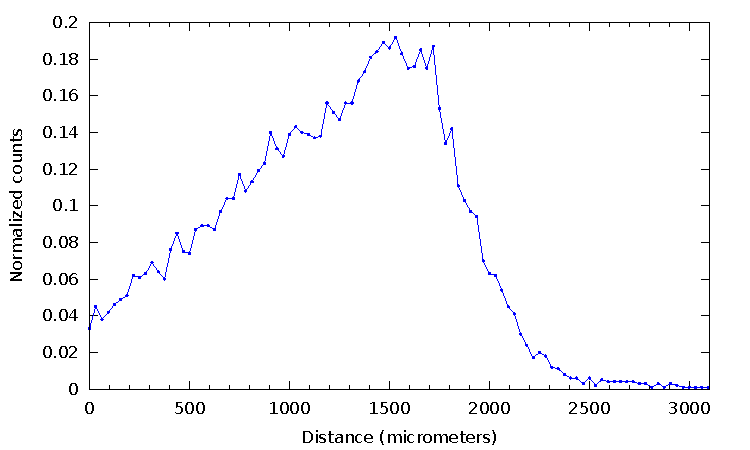
\includegraphics[width=\textwidth]{results/au_sfg_560+800_whitelight}
\caption[White light emission, gold sample.]{White light emission with 560 NOPA beam, gold sample.\label{fig_au_sfg_whitelight}}
\end{figure}

The samples also had a relatively small tolerance for white light emission especially with the XP2SFG setup. Reducing the 800 nm beam with a 0.8 optical density (OD) neutral density filter yielded no emission distinguishable from the substrate. Going down to 0.7 OD there was white light generation, as depicted in figure \ref{fig_au_sfg_whitelight}. Effectively working in a 0.1 OD difference was challenging. Adjusting beam sizes became the best means for controlling the input intensity -- a solution far from optimal. 

This becomes especially apparent when comparing with the figures of references \cite{PhysRevB.84.165316} and \cite{wirth2008second} which elaborate on the models used to determine the different response coefficients based on the empirical data. I asked Junwei Wei about the data we were obtaining and he said that it varied too much from run to run to get any meaningful information out of it, and that it would not fit the current models they had developed.

%%%%%%%%%%%%%%%%%%%%%%%%%%%%%%%%%% Silicon Sample %%%%%%%%%%%%%%%%%%%%%%%%%%%%%%%%%%%%%%%
\section{Silicon Nanoparticles}
The Si sample, although rarely mentioned up until this point, was my hope to connect with the previous work done by the group. I looked at their Si samples and immediately noted that the color was very different -- theirs were light yellowish and mine was dark gray. We speculated on this difference when we observed how flat the transmission curve was as shown in figure \ref{fig_transmission}.

\subsection{Ellipsometry}
We had high hopes for more useful measurements with this sample because of its much better physical state.

\begin{figure}[h]
  \centering
  \subfloat[Graph for $\Psi$.\label{fig_si_ellip_1}]{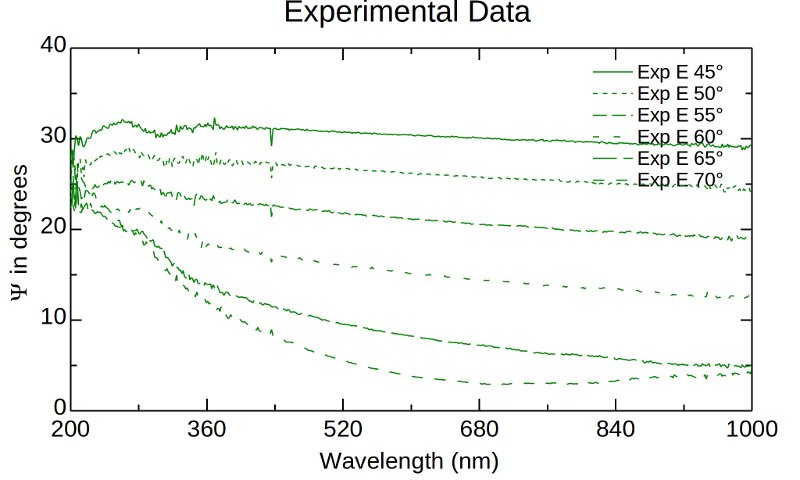
\includegraphics[width=0.5\textwidth]{results/si_ellipsometry_1}}  
  \subfloat[Graph for $\Delta$.\label{fig_si_ellip_2}]{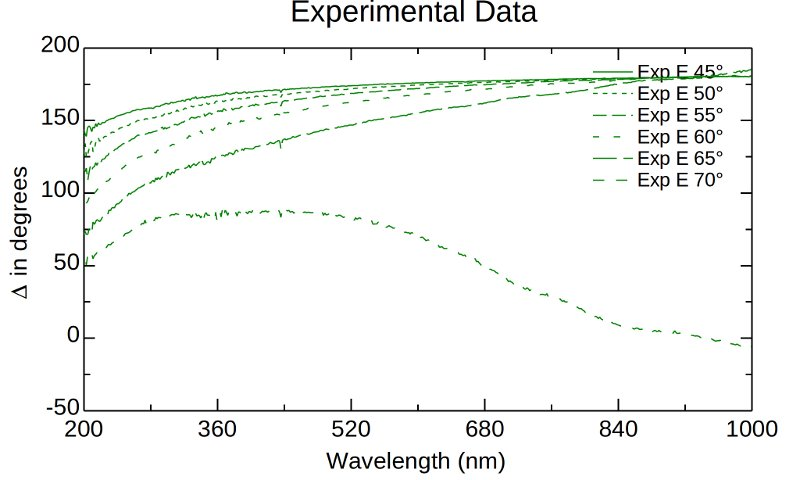
\includegraphics[width=0.5\textwidth]{results/si_ellipsometry_2}}
  \caption[Si ellipsometry.]{Si ellipsometry. Graphs courtesy of Junwei Wei.\label{fig_si_ellip}}
\end{figure}

The data for this sample does not seem to have any meaningful interpretation, just like the gold samples. There appear to be some contribution from the substrate, but not much else.  Reference \cite{PhysRevB.84.165316} demonstrates successful ellipsometric measurements for samples similar to this one. They are consistent with literature and clearly share nothing in common with the results obtained here. The dark grey aspect of the sample may indicate some form of damage to the sample perhaps during annealing or due to environmental aspects or improper handling.

\subsection{XP2SHG and XP2SFG}
Figure \ref{fig_si_shg} was our best SHG run for the Si sample. It is noisy even when compared with the gold samples. It does present the two peak structure but that's where the similarities with previous studies end. Prof. Downer's group reported that XP2SHG enhanced the SHG signal so much that a photon counter was often no longer needed. This was certainly not the case for this sample, with its highest count below 140 photons. The rest of the data produced by this sample was well below this value and did not present even the double peaks.

Figure \ref{fig_si_sfg} is one of only a few SFG runs we did for this sample. Signal intensity was extremely low and looks identical to the substrate contribution.

\begin{figure}[h]
\centering
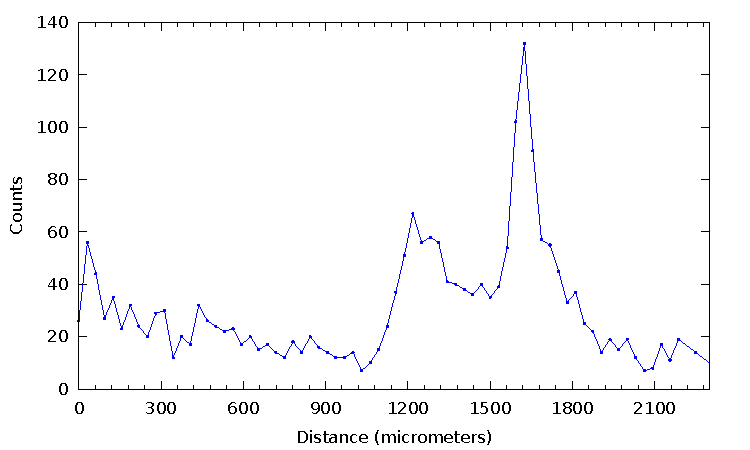
\includegraphics[width=0.85\textwidth]{results/si_shg}
\caption{XP2SHG signal, silicon sample.\label{fig_si_shg}}
\end{figure}

\begin{figure}[H]
\centering
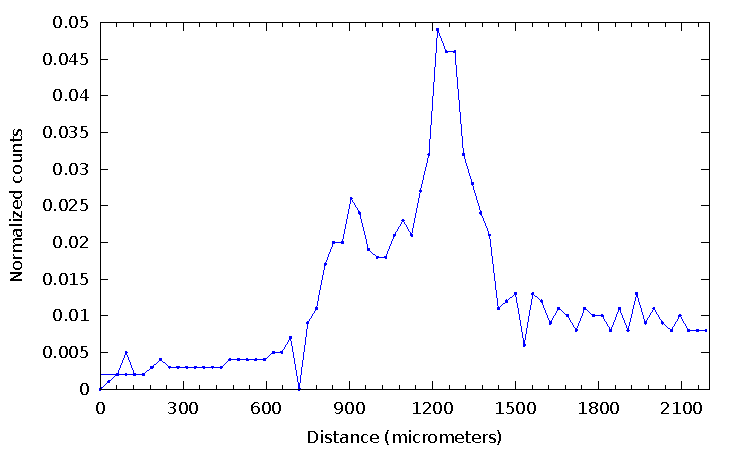
\includegraphics[width=0.85\textwidth]{results/si_sfg_500+800}
\caption{XP2SFG signal, silicon sample.\label{fig_si_sfg}}
\end{figure}

\subsection{Analysis}
I wanted to use this sample as a reference point with the group's previous work, but it became clear from the very beginning that this sample had nothing in common with theirs. After analyzing the linear data we suspected that the sample was most likely damaged in some way. The XP2SHG/SFG runs yielded only a very weak signal compared to the gold samples and to the group's samples. The resulting curves are very inconsistent and ambiguous.

\section{Summary}
We have reviewed all the relevant data for the different samples. Unfortunately the samples were not of good enough quality to yield reliable information. Time constraints and availability did not allow me to obtain different, well characterized, and better samples to redo these measurements. Junwei Wei and Prof. Downer both agreed that these samples had no future for this study and that the data so obtained so far would not yield any meaningful interpretation.

That said, there was a lot learned during this experiment. I review these points and conclude in chapter \ref{chap_conc}.

\chapter{Final Remarks}\label{chap_conc}
\minitoc
\section{Conclusion}
I was able to learn and successfully apply the XP2SHG/SFG technique to a series of nanoparticles that were unfortunately not of sufficient optical quality to yield meaningful results. This was accomplished by using established methods (with the help of very capable people) to study samples that were not properly characterized. The obvious solution to this would have been to use other nanoparticles, but it was very much beyond my possibilities to obtain other samples within the time constraints imposed by my visit to the Femtosecond Spectroscopy group.

My suggestions for a revisionary work are the following.

\begin{description}
\item[Better quality samples.] The scattering problem can be completely eliminated with samples that are in good physical condition.
\item[Well characterized samples.] The purpose of this work was to characterize the nanoparticles via nonlinear spectroscopy. However, these measurements work much better if applied in conjunction with previous studies of the samples, such as TEM scans, linear measurements, etc.
\item[Apply the XP2SFG technique to metallic nanoparticles.] There are few references available on sum frequency studies involving metallic nanoparticles, especially in the two beam configuration. I think that using proper samples with a NOPA in the XP2SFG configuration would provide excellent characterization of the samples and interesting results.
\end{description}

\section{Final Remarks}
I think that every work of experimental science has its fair share of setbacks, complications, and difficulties. Sometimes the work itself can be very difficult or even dangerous. Other times, the work is so cutting edge that problems have to be solved as they come without the help of literature. Regardless of the scope of the work, \emph{all} experimentation is very touch-and-go business -- you arm yourself with the best tools available for the job and hope for the best. This work had its share of complications and setbacks, chief amongst these was the constant breakdown of lasers in both countries. Then, the poor quality of the samples which only came to light after they were in place and ready to be measured. Lastly, the lack of information about the samples did not allow for the systematic study needed to get the most out of this project.

Fortunately, Stephen Jay Gould once said that, ``Honorable errors do not count as failures in science, but as seeds for progress in the quintessential activity of correction.'' With that in mind I summarize what was learned from this.

First, the XP2SHG/SFG technique is fairly unique and specialized even amongst groups that are dedicated to surface optics and nonlinear optical techniques. Learning how this technique works and how it is used will be invaluable for future work in this field. Actually having seen it in use, and then using it for myself in the company of the people who pioneered it was a rewarding and educational experience.

Second, while the results were inconclusive, the types of measurements done on these types of samples are new and unexplored. There is much work to be done with these kinds of materials and I hope that this work can serve as a starting point for other interested scientists. I have no doubt in my mind that better samples would have yielded excellent new results.

Lastly, this entire work helped broaden my knowledge of nonlinear optics in general, as well as the many experimental techniques used everyday by scientists everywhere. Even so, I only possess a very small portion of the ``big picture'' needed to understand every aspect of this work. There is still a lot to be learned about surface optics and nonlinear techniques and I hope that this work, at the very least, will pique the readers' interest on these topics.


%\appendix
%\include{} 

\backmatter
%%%%%%%%%%%%%%%%%%%%%%%%% Select one bibliography style %%%%%%%%%%%%%%%%%%%%%%%%%%%%
%\bibliographystyle{plain}
%\bibliographystyle{abbrv}
%\bibliographystyle{alpha}
\bibliographystyle{unsrt}
\nocite{*} 
\bibliography{base/thesis}

\chapter{Vita}
Sean Anderson was born in San Francisco, California in 1984. Born to restless parents, he spent a good part of his youth traveling between the United States, Mexico, and Guatemala, where his mother is from. Since then, Mexico has never been far from his heart.

He entered the University of Alabama in Hunstville in 2002, under the tutelage of Dr. Don Gregory. In 2006 he graduated magna cum laude with a degree in physics and a minor in mathematics. That same year marked the beginning of a 3 and a half year break to pursue various artistic interests.

He spent most of 2007 dancing tango and photographing Buenos Aires, Argentina. 2008 marked the return to Mexico, where he helped start the family business until 2009.

In 2010 he began his masters degree in optical science at the Centro de Investigaciones en \'Optica in Le\'on, Mexico with Dr. Ram\'on Carriles as his advisor. This thesis marks the culmination of that work and was completed on January 16, 2012.

He is currently continuing on to pursue his Ph.D. in theoretical surface optics with an emphasis in scientific computing with the guidance of Dr. Bernardo Mendoza. His primary interests are the development and usage of free and open source software, GNU/Linux, and parallel computing applied towards solving various scientific problems.
\clearpage
\thispagestyle{empty}

\end{document}
